\chapter{The \alphat Analysis}
\label{ch:analysis}

% **************************** Define Graphics Path **************************
\ifpdf
    \graphicspath{{Chapter5/Figs/Raster/}{Chapter5/Figs/PDF/}{Chapter5/Figs/}}
\else
    \graphicspath{{Chapter5/Figs/Vector/}{Chapter5/Figs/}}
\fi


%********************************** % First Section  *************************************
\section{Analysis Overview}  %Section - 1.1 
\label{sec:selection_analysis_overview}

Analyses searching in the jets and \met final state encounter significant 
backgrounds from SM sources of both genuine and fake \met. Genuine \met 
originates from \ttbar, W and Z boson production, with one or more
neutrinos in the final state. In this analysis background predictions are made
for these processes using 
extrapolations into the signal region from independent, process-specific control
samples, as described in chapter~\ref{ch:background}.
Fake \met predominantly originates from mismeasurements of QCD 
multijet (MJ) production, which is the dominant process in the hadronic
environment
and  phase space considered in this analysis due to it's very large cross
section.  Small inconsistencies in the handling of such large backgrounds or
rare detector effects can therefore 
have a significant impact on an analysis. This background is reduced to an 
entirely negligible level using the dimensionless kinematic variable, \alphat
(described in section~\ref{sec:alphat}).

% OLD
% Analyses searching in the jets and \met final state encounter significant 
% backgrounds from SM sources of both genuine \met, originating from the leptonic 
% decays of W bosons, 
% and fake \met, originating from jet mismeasurement. The \alphat 
% analysis makes predictions for the former using a data-driven transfer factor 
% technique to extrapolate yields from statistically independent control samples 
% into the signal region. However the latter, sources of fake \met from QCD multijet events,
% are reduced to a negligible level using the kinematic 
% variable \alphat.

In this analysis events are binned in exclusive categories of \HT, 
and the multiplicity of jets and b-tagged jets,  
\nj and \nb, as summarised in table~\ref{tab:ht-bins}. Such binning allows for
targeted interpretations across the vast array of
possible simplified model final states, while reducing background yields to a 
minimum.

\begin{table}[ht!]
  \caption{\HT bin lower bounds used for each \nj and \nb category.\label
  {tab:ht-bins}}
  \centering
  \small
  \begin{tabular}{ lrrrrrrrrrrr }
    \hline
    \hline
    (\nj,\nb)       & \multicolumn{11}{c}{\HT bins (\gev)} \\
    \hline
    (2-3,0)           & 200 & 275 & 325 & 375 & 475 & 575 & 675 & 775 & 875 & 975 & $>$1075  \\
    (2-3,1)           & 200 & 275 & 325 & 375 & 475 & 575 & 675 & 775 & 875 & 975 & $>$1075  \\
    (2-3,2)           & 200 & 275 & 325 & 375 & 475 & 575 & 675 & 775 & $>$875   & \multicolumn{2}{c}{} \\
%    (2-3,3)          & 200 & 275 & 325 & 375 & 475 & 575 & 675 & 775 & $>$875   & \multicolumn{2}{c}{} \\
    ($\geq$4,0)       & 200 & 275 & 325 & 375 & 475 & 575 & 675 & 775 & 875 & 975 & $>$1075  \\
    ($\geq$4,1)       & 200 & 275 & 325 & 375 & 475 & 575 & 675 & 775 & 875 & 975 & $>$1075  \\
    ($\geq$4,2)       & 200 & 275 & 325 & 375 & 475 & 575 & 675 & 775 & $>$875   & \multicolumn{2}{c}{} \\
    ($\geq$4,3)       & 200 & 275 & 325 & 375 & 475 & 575 & 675 & 775 & $>$875   & \multicolumn{2}{c}{} \\
    ($\geq$4,$\geq$4) & 200 & 275 & 325 & $>$375   & \multicolumn{7}{c}{}    \\
    \hline
    \hline
  \end{tabular}
\end{table}

The main analysis search region is described in the remainder of this chapter.


\subsection{The \alphat kinematic variable}
\label{sec:alphat}

% QCD multijet (MJ) events dominate the SM background in any search with multiple jets 
% in the final state. Jet energy mismeasurements in a 
% purely QCD MJ event can lead to non-negligible amounts of \mht, therefore 
% passing the signal selection.
Attempting to accurately measure the QCD contribution to the total background is
particularly challenging given the hadronic environment of the LHC and the lack
of precise measurements and calculations of the large multijet cross sections
involved. As an
alternative approach, the goal of this analysis is to reduce QCD down to an
entirely negligible levels with respect to background processes with genuine
\met, achieved through the use of the dimensionless kinematic
variable, \alphat. The di-jet variable
$\alpha$ was first proposed by Randall et al. in 2008 \cite{Randall:2008rw},
and later translated into the transverse plane for use with LHC analyses
\cite{CMS:2008vya, CMS-PAS-SUS-09-001}.
\alphat is defined for di-jets as:
% 
\begin{equation}
\alphat = \frac{ \sqrt{E_T^{j_2}/E_T^{j_1}} }{ \sqrt{2(1-cos(\Delta \phi))} } ,
\label{eq:alphat_di-jet}
\end{equation}
% 
where $E_T^{j_1}$ and $E_T^{j_2}$ are the reconstructed transverse energies of 
the first and second jets respectively, and $\Delta \phi$ is the separation 
between the two jets in the $\phi$ plane.

A perfectly measured di-jet event containing back to back jets in $\phi$ of equal energy will
have an \alphat value of 0.5, whereas 
events with \met originating from jet energy mismeasurements will have values of $\alphat<0.5$.
Only events containing sources of genuine \met, whether from SM or BSM sources,
can have values of $\alphat > 0.5$.
% 
% \begin{equation}
% \alphat = \frac{E_T^{j_2}}{M_T} = \frac{\sqrt{}}
% \label{eq:alphat_di-jet}
% \end{equation}
% 
% where $E_T^{j_2}$ is the transverse energy of the less energetic jet and $M_T$ 
% is the transverse mass of the di-jet system, defined as:
% 
% \begin{equation}
% M_T = \sqrt{\bigg(\sum^2_{i=1}{E_T^{j_i}}\bigg)^2 - \bigg(\sum^2_{i=1}{p_x^{j_i}}\bigg)^2 - \bigg(\sum^2_{i=1}{p_y^{j_i}}\bigg)^2}
% \label{eq:mt}
% \end{equation}
% 
% where $E_T^{j_i}$, $p_x^{j_i}$ and $p_y^{j_i}$ are the transverse energy and 
% transverse momentum in the $x$ and $y$ planes, for the jet $j_i$.

The \alphat variable can be generalised to an n-jet case by considering the event as a 
pseudo-di-jet system, constructing each pseudo-jet such that the difference in \HT
between each pseudo-jet system, \deltaHT, is minimised. \alphat then takes the 
form:
% 
\begin{equation}
\alphat = \frac{1}{2} \times \frac{\HT-\deltaHT}{\sqrt{\HT^2 - \mht^2}} = 
\frac{1}{2} \times \frac{1-\frac{\deltaHT}{\HT}}{\sqrt{1 - \big(\frac{\mht}
{\HT}\big)^2}}.
\label{eq:alphat_njet}
\end{equation}
% 

The \alphat variable introduces a correlation between the two variables of \mht
and \deltaHT. This relationship is demonstrated in figure~\ref{fig:alphat_corr}
by the black contours of constant \alphat. Different physics processes
will populate various regions of this plane, as shown in the MC study in
figure~\ref{fig:alphat_corr}. Most notably QCD exhibits a strong
correlation between the two variables at low \alphat values
(figure~\ref{fig:alphat_corr_qcd}), while processes with real \met break this
correlation, sitting also at higher values of \alphat
(figures~\ref{fig:alphat_corr_zinv} and \ref{fig:alphat_corr_t2cc}).

\begin{figure}[t!]
  \centering
  \begin{subfigure}[t]{.46\textwidth}
    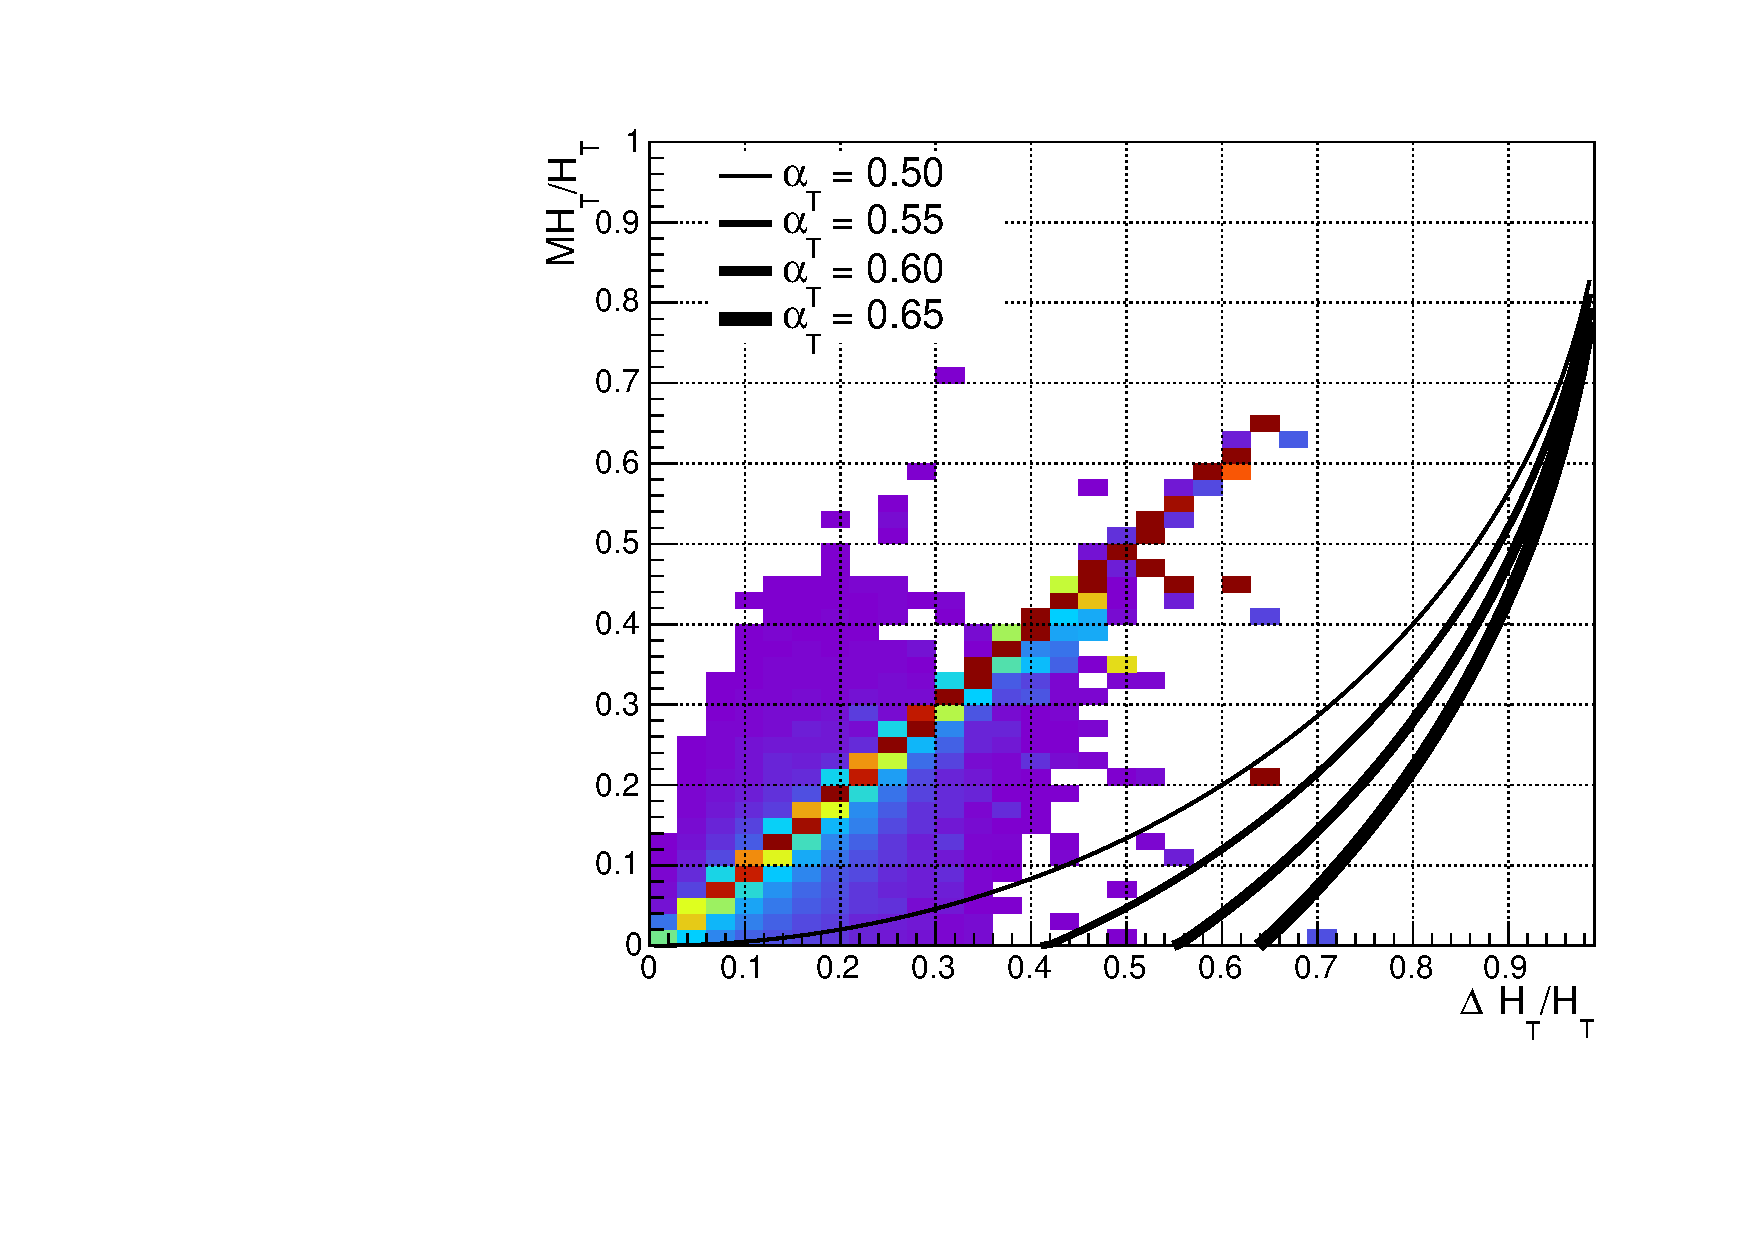
\includegraphics[width=\textwidth]{Figs/alphat/alphat_correlation_QCD.pdf}
    \caption{QCD}
    \label{fig:alphat_corr_qcd}
  \end{subfigure}
  \begin{subfigure}[t]{.46\textwidth}
    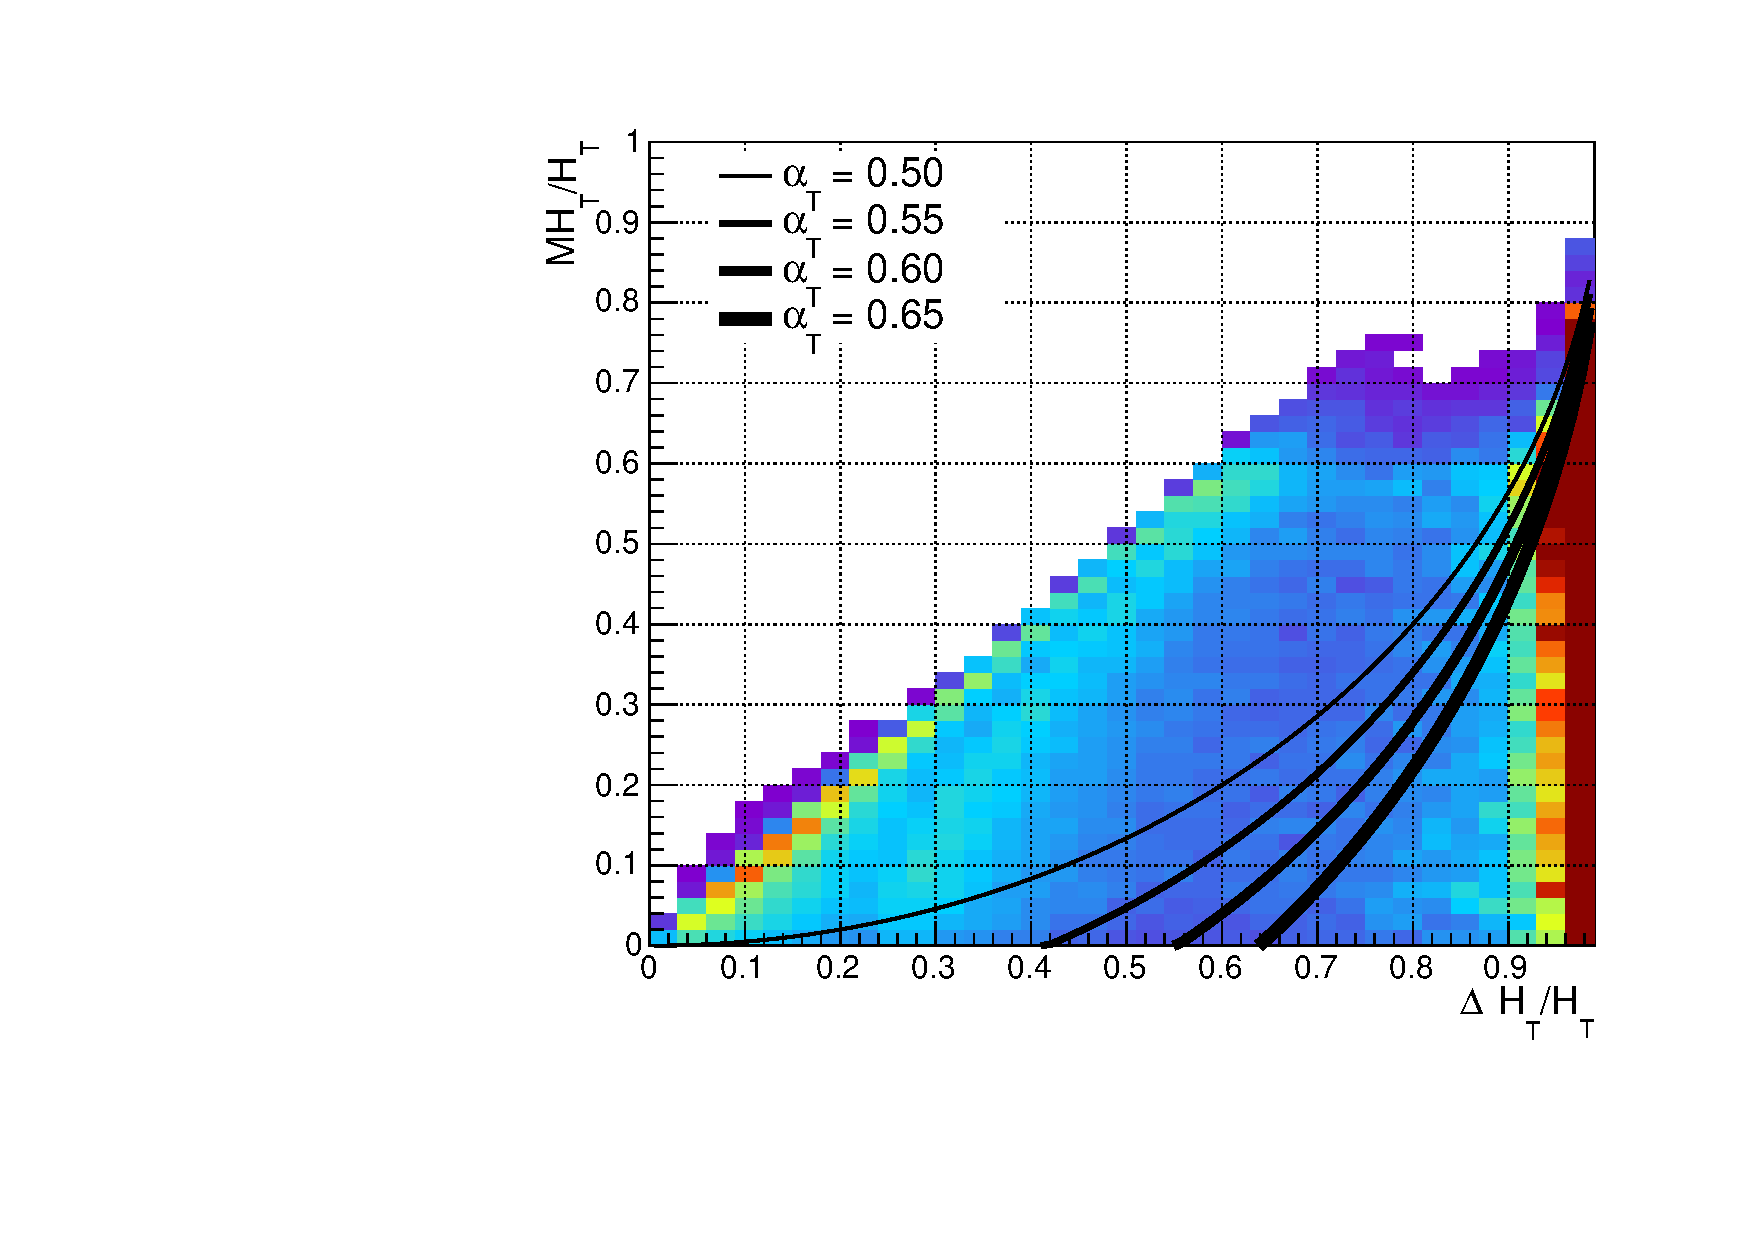
\includegraphics[width=\textwidth]{Figs/alphat/alphat_correlation_Zinv.pdf}
    \caption{\zinv}
    \label{fig:alphat_corr_zinv}
  \end{subfigure}\\
  \begin{subfigure}[t]{.46\textwidth}
    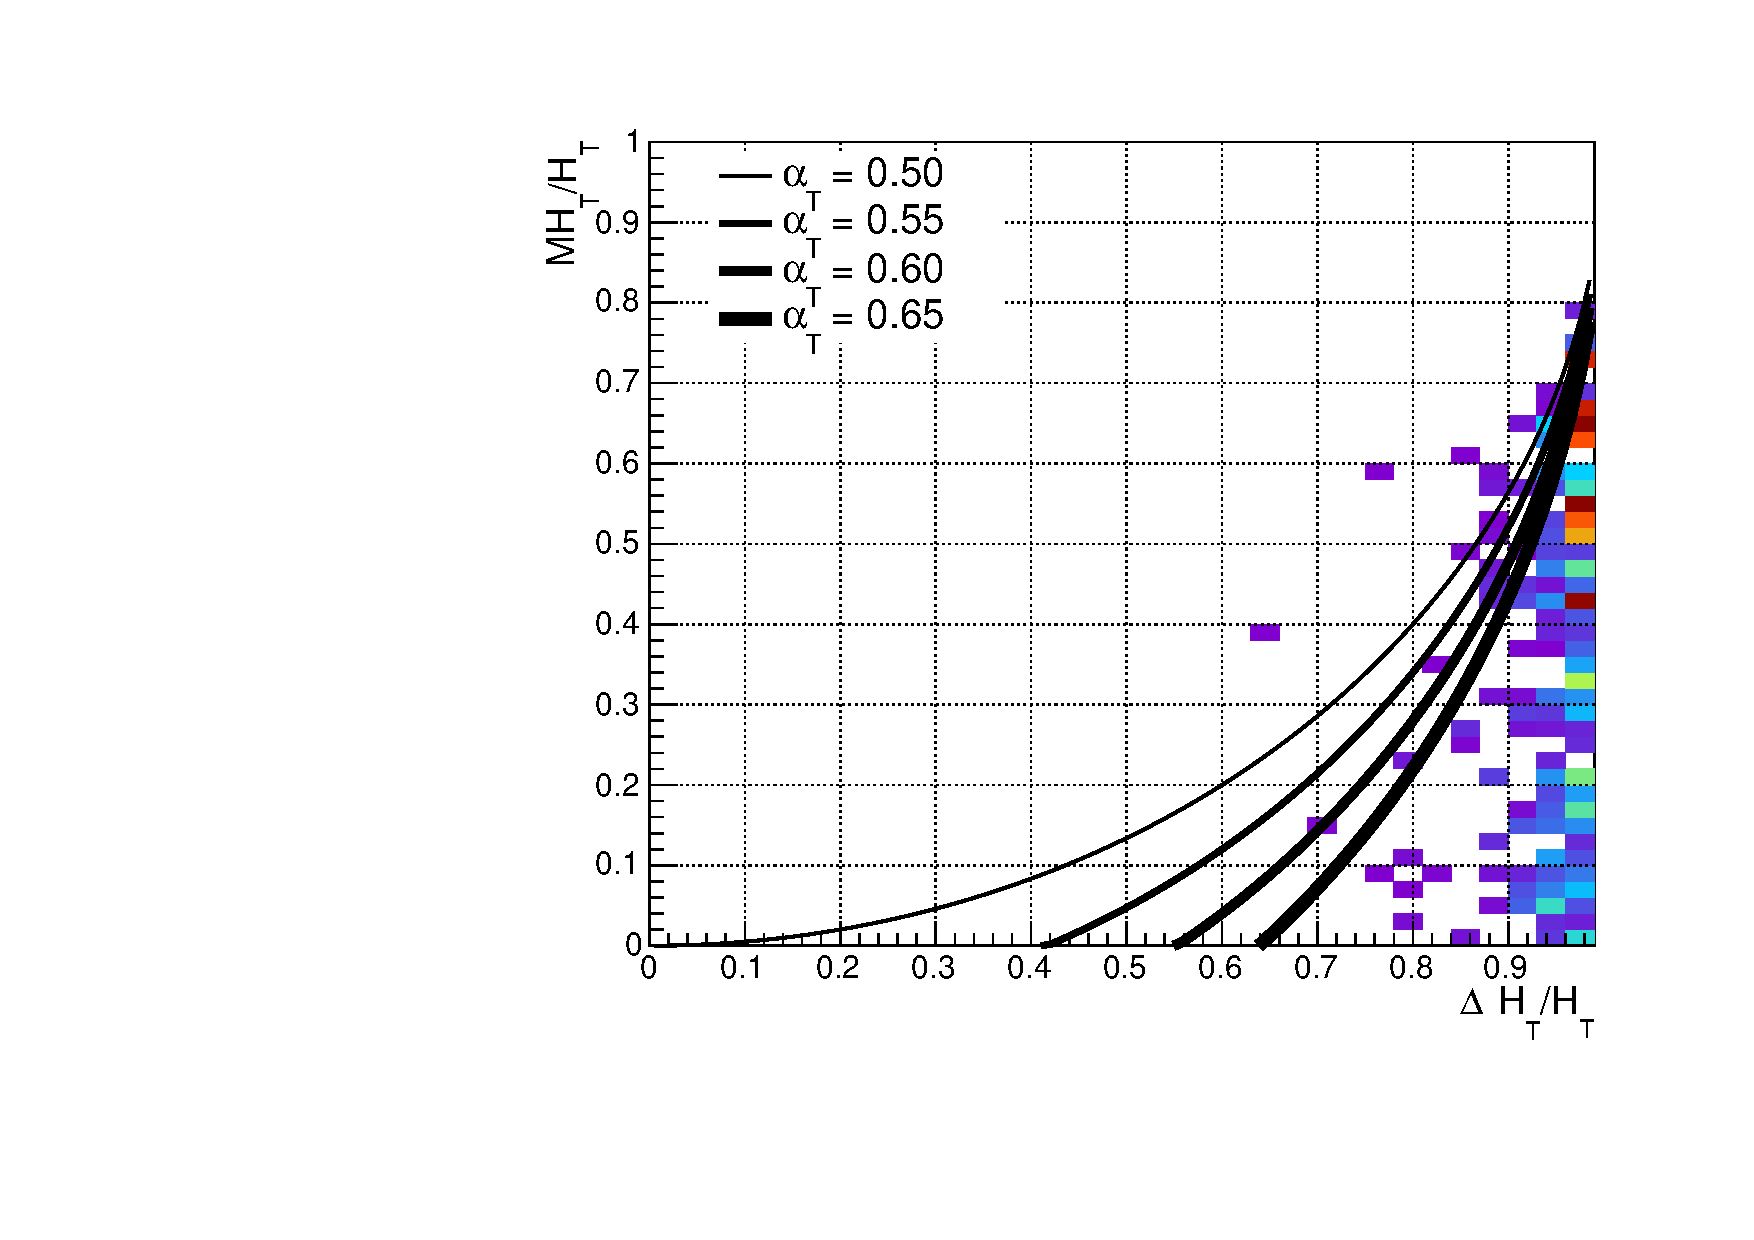
\includegraphics[width=\textwidth]{Figs/alphat/alphat_correlation_T2cc_250_240.pdf}
    \caption{\texttt{T2cc} (250, 240)}
    \label{fig:alphat_corr_t2cc}
  \end{subfigure}
  \caption{The correlation between \mht and \deltaHT for MC samples of QCD,
  \zinv and an example SUSY signature \texttt{T2cc} ($m_{\sTop} = 250$~\gev,
  $m_{\chiz} = 240$~\gev). Contours of constant \alphat are shown in black.
  Each axis is normalised according to the events \HT.}
  \label{fig:alphat_corr}
\end{figure}

Through the requirement of \alphat in a given region of \HT, a certain missing
energy threshold is implied. Figure~\ref{fig:alphat_mht_corr} shows this, for
the assumption of \deltaHT = 0 - an assumption which yields the minimum \mht
values. Given this correlation, the implicit missing energy threshold can be
maintained across the \HT range by lowering \alphat thresholds in the high \HT
region.

\begin{figure}
  \centering
  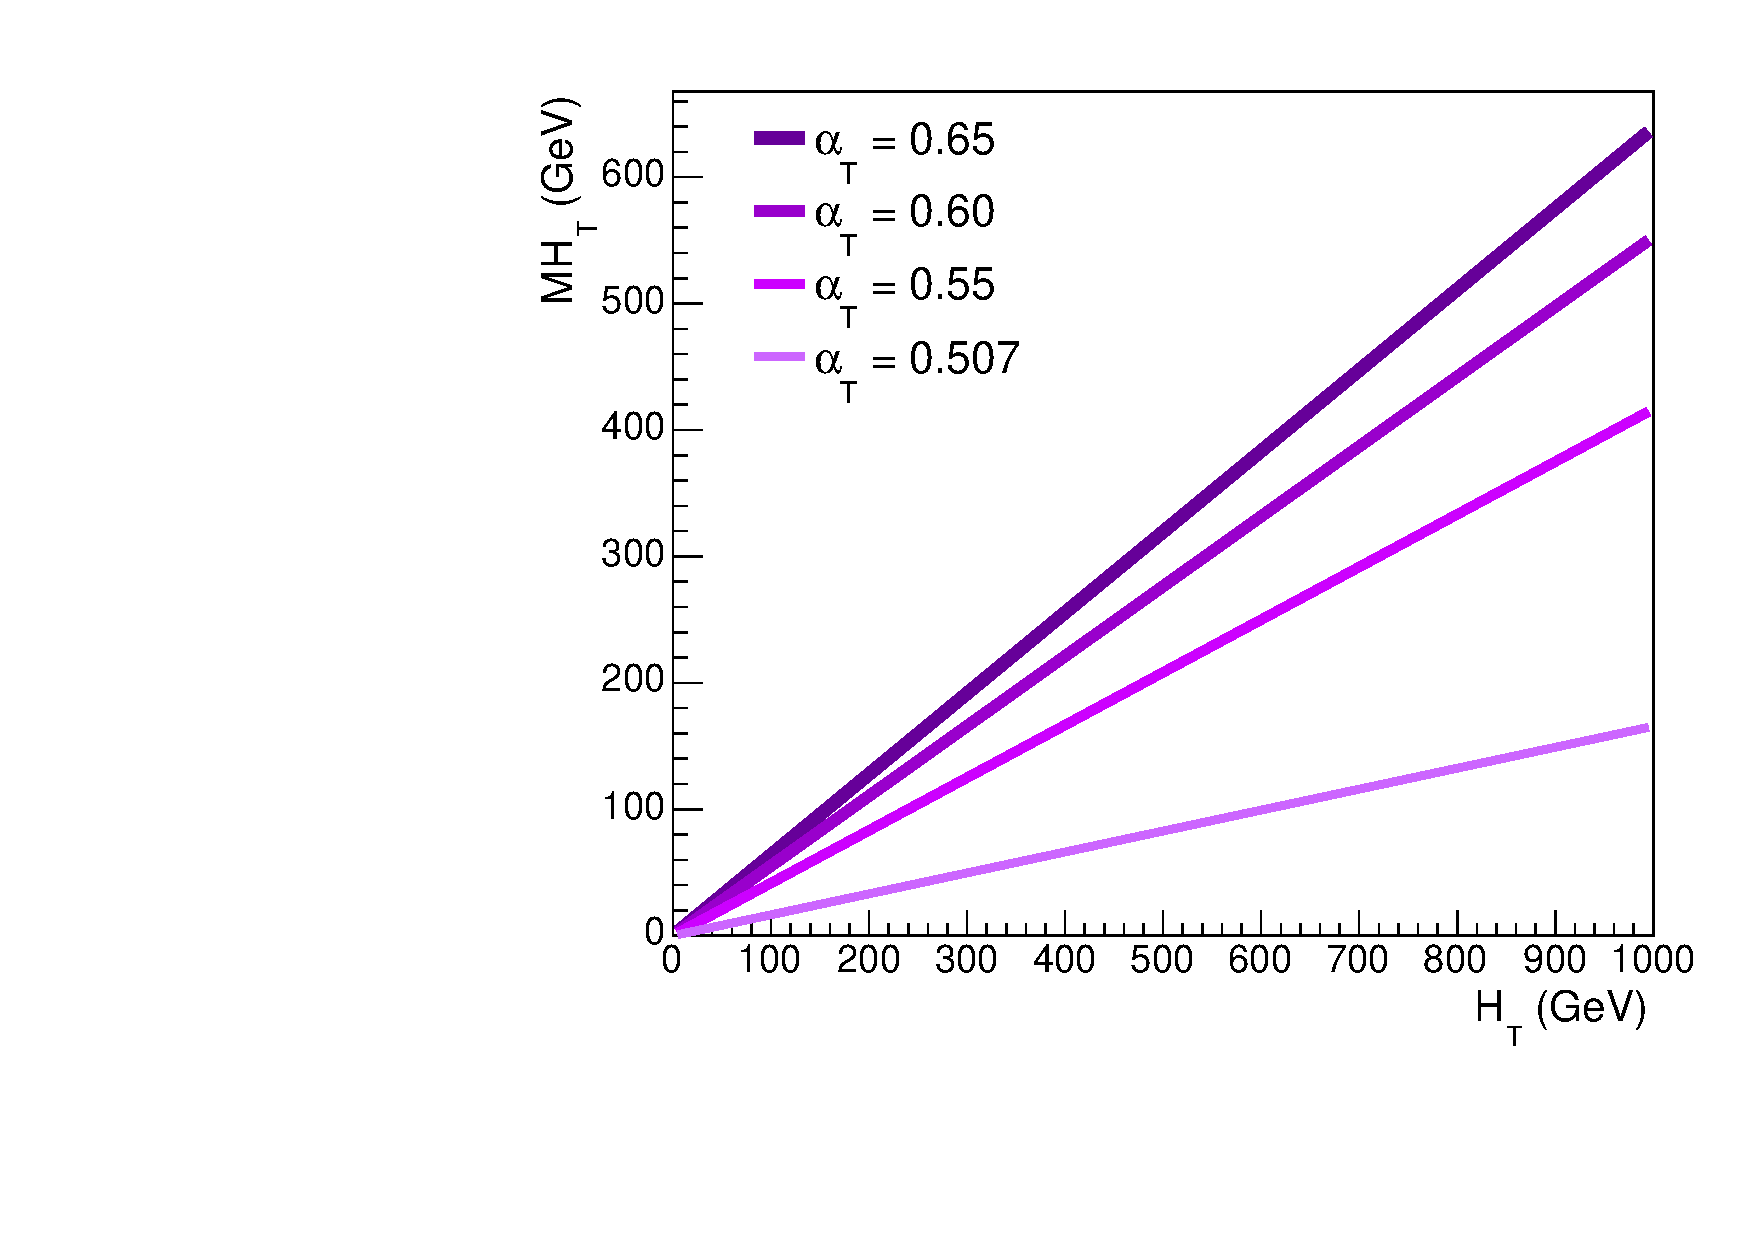
\includegraphics[width=0.7\textwidth]{Figs/alphat/mht_correlation.pdf}
  \caption{The correlation between \HT and \mht for different \alphat values,
  with the assumption of \deltaHT = 0.}
  \label{fig:alphat_mht_corr}
\end{figure}

%********************************** % First Section  *************************************

\section{Standard Model Backgrounds}
\subsection{Genuine \met}
The dominant Electroweak (EWK) source of genuine missing energy comes from
Z-boson production where the Z decays
to neutrinos, \zinv, with associated jet production. This source of background
is considered irreducible.

Events containing leptonic decays of W bosons, \wlnu, originating either
from direct W production, or via the decay of a top quark from \ttbar 
production, are sources of genuine 
missing energy due to the presence of a weakly interacting neutrino which
evades detection. Such events are vetoed in the signal
region due to the presence of a 
lepton, however if the lepton is missed leptonic W decays 
can pass the signal selection, forming a significant SM background.

% While lepton and photon vetoes employed in the signal region suppress 
% significant amounts of background from events with neutrinos, such events can 
% still persist if, for example, the lepton is not identified.
% Such processes are predominantly from \ttbar or W-boson production, where the 
% W decays via \wlnu. If the lepton is `lost' and evades our 
% lepton vetoes, significant missing energy can be produced not only from missing 
% the lepton, but from the presence of the neutrino. When such processes are accompanied 
% by associated jet production they are then able to pass our signal region selection.

Leptons can be `lost' for a variety different reasons, but ultimately for failing
the lepton ID criteria. There are numerous potential causes, the 
most prevalent being soft-leptons below the ID's \Pt threshold or non-isolated
leptons
which pass the ID quality cuts but fail the isolation requirement.


% \emph{move to selection section}
% Events containing a Single Isolated Track (SIT) are vetoed from the signal 
% region. This tracker based veto is particularly useful for vetoing additional events 
% that contain leptons which have failed our lepton ID requirements entirely, and 
% are therefore not considered by the leptonic vetoes. Additionally, the veto also
% removes background contributions from single-pronged hadronic decays of $\tau$
% leptons.

% While originally designed to target hadronically decaying tau leptons, 
% this requirement reduces the remaining lost-lepton backgrounds also.

Following the hadronic selection requirements (outlined in
section~\ref{sec:selec_crit}),
any remaining contributions from SM EWK backgrounds are estimated using a 
fully data-driven transfer factor technique, described in detail in
Section~\ref{sec:background_overview}.

\subsection{Fake \met}

As mentioned previously, the dominant source of background for analyses 
searching for a multijet final state is from QCD. A fully-measured QCD event 
would consist of multiple jets balancing each other in all planes, however in 
order to enter the signal region, an event must contain missing energy, 
\mht (equivalent to \met in all-hadronic events).

The most common way for a balanced multijet (MJ) event to gain \mht occurs if
one
or more of the jets are mismeasured, such that their vectorial sum then leads to non-zero
\mht. This can occur due to detector issues, or due to stochastic fluctuations
within
the inherant jet-resolution of the 
detector. The former is protected against by the \met filters summarised in 
table~\ref{tab:met_filters} and using a filter to remove events
affected by non-functioning or damaged regions of the ECAL system, where 
events are vetoed if they contain significant energy deposits within a given 
distance from a known problematic region. The latter is dealt with using a
cut on the \alphat variable where 
events with fake missing energy signatures give values $<0.5$.

QCD MJ events can also appear to contain non-zero missing energy 
due to the threshold requirements of jets. If an event contains 
one or more jets below the analysis threshold, then the 
event is measured as imbalanced and containing \mht. Events such as these are largely 
removed with the \alphat requirement, however in addition a requirement is made on the
ratio \mhtmet.

Residual QCD cleaning details are given later in section~\ref{sec:qcd_cleaning}.

% Finally, it is also possible for rare instrumentation effects to lead to jet 
% energy
% mismeasurements. To protect against this, a suite of MET filters are defined by 
% the JetMET \emph{POG}, and are applied to all selections.


\section{Signal Triggers}

Events are collected at the HLT using a dedicated suite of
signal triggers. For an event to pass the trigger
requirements, it must exceed both a \HT and an \alphat threshold. Trigger rate 
can be maintained by varying the
threshold on each of these independent requirements, as shown in
Table~\ref{tab:sig_trigs}. Each \HT bin in the analysis is seeded by a
specific signal
trigger, with a 25~\gev offset between online and offline \HT, with the
exception of the 200~\gev bin.

Exclusively for this analysis, the additional `Parked' trigger 
\\\verb!HT200_AlphaT0p57! is included, seeding the new \HT> 200~\gev bin. Such a low
threshold allows sensitivity to be maintained for softer physics signatures, such
as those expected from compressed spectra SUSY decays studied in this work.

\begin{table}[!ht]
  \caption{Signal triggers, the L1 seed triggers and their efficiencies measured
  for per \HT and \nj category.}
  \label{tab:sig_trigs}
  \centering
  \scriptsize
  \begin{tabular}{ cccccc }
    \hline
    \hline
    Offline \HT       & Offline \alphat & L1 seed (\verb!L1_?!)         & Trigger (\verb!HLT_?!)  & \multicolumn{2}{c}{Efficiency (\%)}          \\ [0.5ex]
    region (\gev)         & threshold       & (highest thresholds)          &                         & $2 \leq \nj \leq 3$ & $\nj \geq 4$       \\ [0.5ex]
    \hline
    $200 < \HT < 275$ & 0.65            & \verb!DoubleJetC64!           & \verb!HT200_AlphaT0p57! & $81.8^{+0.4}_{-0.4}$  & $78.9^{+0.3}_{-0.4}$ \\
    $275 < \HT < 325$ & 0.60            & \verb!DoubleJetC64!           & \verb!HT200_AlphaT0p57! & $95.2^{+0.3}_{-0.4}$  & $90.0^{+1.2}_{-1.3}$ \\
    $325 < \HT < 375$ & 0.55            & \verb!DoubleJetC64 OR HTT175! & \verb!HT300_AlphaT0p53! & $97.9^{+0.3}_{-0.3}$  & $95.6^{+0.9}_{-1.0}$ \\
    $375 < \HT < 475$ & 0.55            & \verb!DoubleJetC64 OR HTT175! & \verb!HT350_AlphaT0p52! & $99.2^{+0.2}_{-0.2}$  & $98.7^{+0.5}_{-0.7}$ \\
    $\HT > 475$       & 0.55            & \verb!DoubleJetC64 OR HTT175! & \verb!HT400_AlphaT0p51! & $99.8^{+0.1}_{-0.3}$  & $99.6^{+0.3}_{-0.7}$ \\
    \hline
    \hline
  \end{tabular}
\end{table}

Trigger efficiencies are measured using an unbiased single-muon reference
trigger,
\\\verb!HLT_IsoMu24_eta2p1!, via a muon tag and probe method where a
single-muon is selected and then subsequently ignored from the analysis when 
calculating event level variables such as \HT, \mht and \alphat. Efficiencies 
are measured for each \HT bin and for each \nj category, as summarised in 
table~\ref{tab:sig_trigs}. Example trigger `turn-on' curves are shown for the 3 
lowest \HT bins in figures~\ref{fig:eff_alphat_le3j} and \ref{fig:eff_alphat_ge4j}.
The curves are shown both differentially and cumulatively, to show the
efficiency for events of a given \alphat value and above an \alphat threshold
respectively.
Across the higher \HT  bins the triggers are measured as fully efficient.
Inefficiencies in the low \HT bins are
understood as being due to the relatively high threshold L1 seed trigger used
for this region, in order to maintain
low rates in the high PU environment encountered throughout \runone. Lower 
efficiencies are also observed in the \njhigh category attributed to the presence of 
softer jets, as an increased number of jets must equate to the same total \HT 
requirement of the bin.

% \afterpage{%
\begin{figure}[p!]
  \centering
    \begin{subfigure}[b]{0.48\textwidth}
      
\includegraphics[width=\textwidth,page=11, trim=0 0 0 20, clip=true]{figures/trigger/HT200_275_73_73_36_AlphaT_le3j_RunAtFNAL}
      \caption{Differential, $200 < \HT < 275 $~\gev}
    \end{subfigure}
    \begin{subfigure}[b]{0.48\textwidth}
      
\includegraphics[width=\textwidth,page=18, trim=0 0 0 20, clip=true]{figures/trigger/HT200_275_73_73_36_AlphaT_le3j_RunAtFNAL}
      \caption{Cumulative, $200 < \HT < 275 $~\gev}
    \end{subfigure} \\
    \vspace{0.5cm}\begin{subfigure}[b]{0.48\textwidth}
      
\includegraphics[width=\textwidth,page=11, trim=0 0 0 20, clip=true]{figures/trigger/HT275_325_73_73_36_AlphaT_le3j_RunAtFNAL}
      \caption{Differential, $275 < \HT < 325 $~\gev}
    \end{subfigure}
    \begin{subfigure}[b]{0.48\textwidth}
      
\includegraphics[width=\textwidth,page=18, trim=0 0 0 20, clip=true]{figures/trigger/HT275_325_73_73_36_AlphaT_le3j_RunAtFNAL}
      \caption{Cumulative, $275 < \HT < 325 $~\gev}
    \end{subfigure} \\
    \vspace{0.5cm}\begin{subfigure}[b]{0.48\textwidth}
      
\includegraphics[width=\textwidth,page=11, trim=0 0 0 20, clip=true]{figures/trigger/HT325_375_86_86_43_AlphaT_le3j_RunAtFNAL}
      \caption{Differential, $325 < \HT < 375 $~\gev}
    \end{subfigure}
    \begin{subfigure}[b]{0.48\textwidth}
      
\includegraphics[width=\textwidth,page=18, trim=0 0 0 20, clip=true]{figures/trigger/HT325_375_86_86_43_AlphaT_le3j_RunAtFNAL}
      \caption{Cumulative, $325 < \HT < 375 $~\gev}
    \end{subfigure} \\
  
    \caption{\label{fig:eff_alphat_le3j}
      Differential (left) and cumulative (right) efficiency turn-on curves for 
      the signal triggers, for the three lowest \HT bins and \njlow.}
\end{figure}
% \clearpage
% }

% \afterpage{%
\begin{figure}[p!]
  \centering
    \begin{subfigure}[b]{0.48\textwidth}
      
\includegraphics[width=\textwidth,page=11]{figures/trigger/HT200_275_73_73_36_AlphaT_ge4j_RunAtFNAL}
      \caption{Differential, $200 < \HT < 275 $~\gev}
    \end{subfigure}
    \begin{subfigure}[b]{0.48\textwidth}
      
\includegraphics[width=\textwidth,page=18]{figures/trigger/HT200_275_73_73_36_AlphaT_ge4j_RunAtFNAL}
      \caption{Cumulative, $200 < \HT < 275 $~\gev}
    \end{subfigure} \\
    \begin{subfigure}[b]{0.48\textwidth}
      
\includegraphics[width=\textwidth,page=11]{figures/trigger/HT275_325_73_73_36_AlphaT_ge4j_RunAtFNAL}
      \caption{Differential, $275 < \HT < 325 $~\gev}
    \end{subfigure}
    \begin{subfigure}[b]{0.48\textwidth}
      
\includegraphics[width=\textwidth,page=18]{figures/trigger/HT275_325_73_73_36_AlphaT_ge4j_RunAtFNAL}
      \caption{Cumulative, $275 < \HT < 325 $~\gev}
    \end{subfigure} \\
    \begin{subfigure}[b]{0.48\textwidth}
      
\includegraphics[width=\textwidth,page=11]{figures/trigger/HT325_375_86_86_43_AlphaT_ge4j_RunAtFNAL}
      \caption{Differential, $325 < \HT < 375 $~\gev}
    \end{subfigure}
    \begin{subfigure}[b]{0.48\textwidth}
      
\includegraphics[width=\textwidth,page=18]{figures/trigger/HT325_375_86_86_43_AlphaT_ge4j_RunAtFNAL}
      \caption{Cumulative, $325 < \HT < 375 $~\gev}
    \end{subfigure} \\
  
    \caption{\label{fig:eff_alphat_ge4j}
      Differential (left) and cumulative (right) efficiency turn-on curves for 
      the signal triggers, for the three lowest \HT bins and \njhigh.}
\end{figure}
% \clearpage
% }

All triggers were present throughout \runone, however the 
\\\verb!HLT_HT200_AlphaT0p57! trigger was used as part of the `Parked' data
stream which was reconstructed at a later date, following the active data-taking
period. During data-taking triggers may have `prescale' factors applied to them 
such that only every $n$ triggered events are actually recorded, however all of
the signal triggers remained without a prescale for the entirety of the 8 \tev
data-taking.


\section{Selection Criteria}
\label{sec:selec_crit}

Event selection requirements for the hadronic signal region are chosen with an
aim to
maintain sensitivity to hadronically decaying sparticle production, while 
rejecting as many QCD-type processes as possible. To do so, requirements are 
made on:

\begin{table}[b!]
  \caption{Jet \Et and \alphat thresholds per \HT bin.
  \label{tab:analysis_thresholds}}
  \centering
  \small
  \begin{tabular}{ lcccc }
    \hline
    \hline
    \HT bin        & 200--275 & 275--325 & 325--375 & $>$375 \\
    \hline
    Lead jet (\gev)       & 73.3     & 73.3     & 86.7     & 100.0  \\
    Second jet (\gev)     & 73.3     & 73.3     & 86.7     & 100.0  \\
    All other jets (\gev) & 36.7     & 36.7     & 43.3     & 50.0   \\
    \hline
    \alphat        & 0.65     & 0.60     & 0.55     & 0.55    \\
    \hline
    \hline
  \end{tabular}
\end{table}

% \begin{table}[b]
%   \caption{\alphat thresholds per \HT bin.\label{tab:alphat_thresholds}}
%   \centering
%   \footnotesize
%   \begin{tabular}{ lccc }
%     \hline
%     \hline
%     \HT bin        & 200--275 & 275--325 & $>$325 \\
%     \hline
%     Lead jet       & 0.65     & 0.60     & 0.55  \\
%     \hline
%     \hline
%   \end{tabular}
% \end{table}


\begin{description}
\item[Jets]
Events are required to contain at least two jets with
$\HT > 200$~\gev, to ensure the presence of significant hadronic activity.
They are categorised by \HT, with jet \Pt
requirements on the two leading and the remaining additional jets separately.
The jet \Pt thresholds vary as a function of the \HT bin of the event, as shown in
Table~\ref{tab:analysis_thresholds}, in order to maintain a similar kinematic
phase space throughout the \HT range.

\item[Leptons]
Any events containing leptons are vetoed to ensure only hadronic events
are considered, thereby suppressing events with genuine \met from leptonic decays to
neutrinos such as \wlnu.

\item[Photons]
Events containing photons are vetoed, for similar reasons as the leptonic 
vetoes, in order to maintain a purely hadronic environment.

\item[Single Isolated Tracks]
Events containing a Single Isolated Track (SIT) are vetoed from the signal 
region. This tracker based veto is particularly useful for vetoing additional events 
that contain leptons which have failed our lepton ID requirements entirely and 
are therefore not considered by the leptonic vetoes. Additionally, the veto also
removes background contributions from single-pronged hadronic decays of $\tau$
leptons.

\item[Event]
The topology of the event is required to pass a threshold of at least $\alphat >
0.55$, a requirement which itself varies as a function of the \HT category being
considered, always chosen such that the signal triggers are in the efficiency
plateau, as summarised in table~\ref{tab:analysis_thresholds}. While no
absolute \met requirement is made, the cut on
\alphat imposes an implied threshold, which maintains the analysis'
sensitivity to very low regions of \met as shown by figure~\ref{fig:alphat_mht_corr}.

\end{description}

A breakdown of the EWK background 
composition is shown in Figure~\ref{fig:background_decomp}, split into the main 
categories of \zinv, \wj, \ttbar and all remaining residual backgrounds, such as
single top quark, diboson and Drell-Yann processes.

\begin{figure}[hb!]
\centering
\hspace{0cm}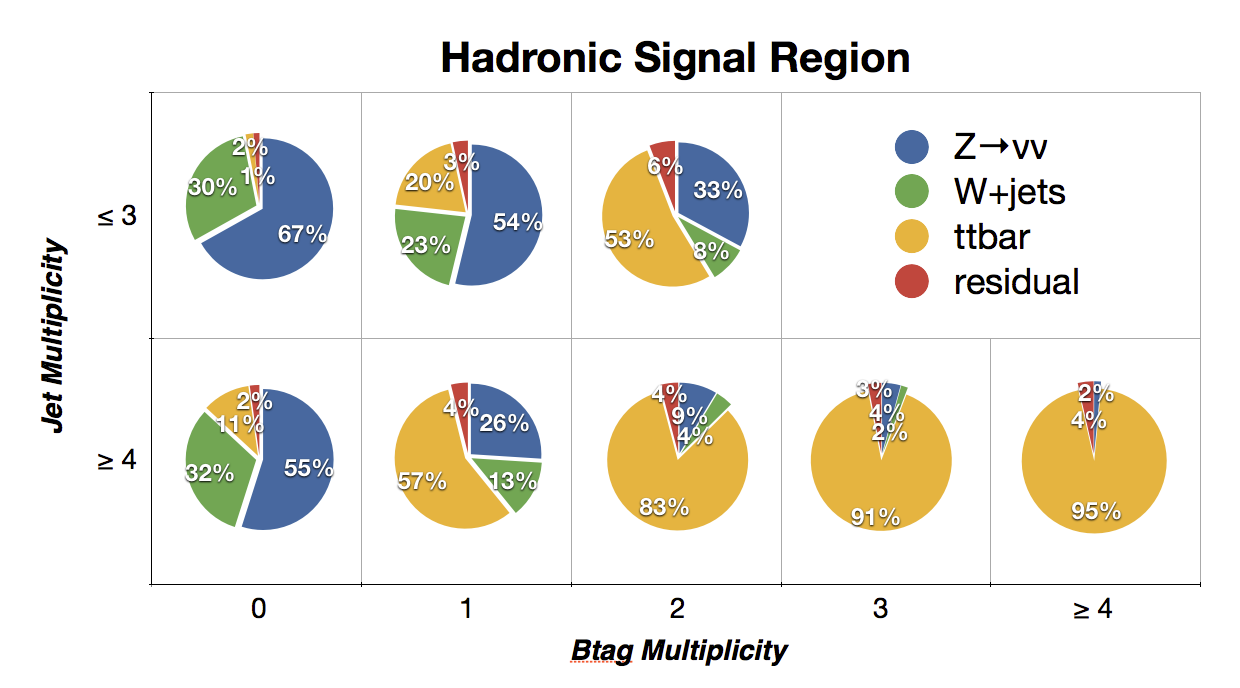
\includegraphics[width=0.9\textwidth, trim=0 00 0 0, clip=true]
{Figs/ra1_had_bg_comp_v3.png}
\caption{The breakdown of the total electroweak background into component
processes as a function of \nj and \nb, for \HT>200~\gev.}
\label{fig:background_decomp}
\end{figure}

\section{Residual QCD cleaning}
\label{sec:qcd_cleaning}

While the \alphat requirement removes many orders of magnitude of QCD events,
there still exist scenarios in which these events may pass the signal region
selection. Accordingly, further requirements are made to ensure the search
region is free of any residual QCD contamination.

\subsection{Multiple jets below threshold}
\label{sec:qcd_cleaning_below_thresh}

\begin{figure}[ht!]
\centering
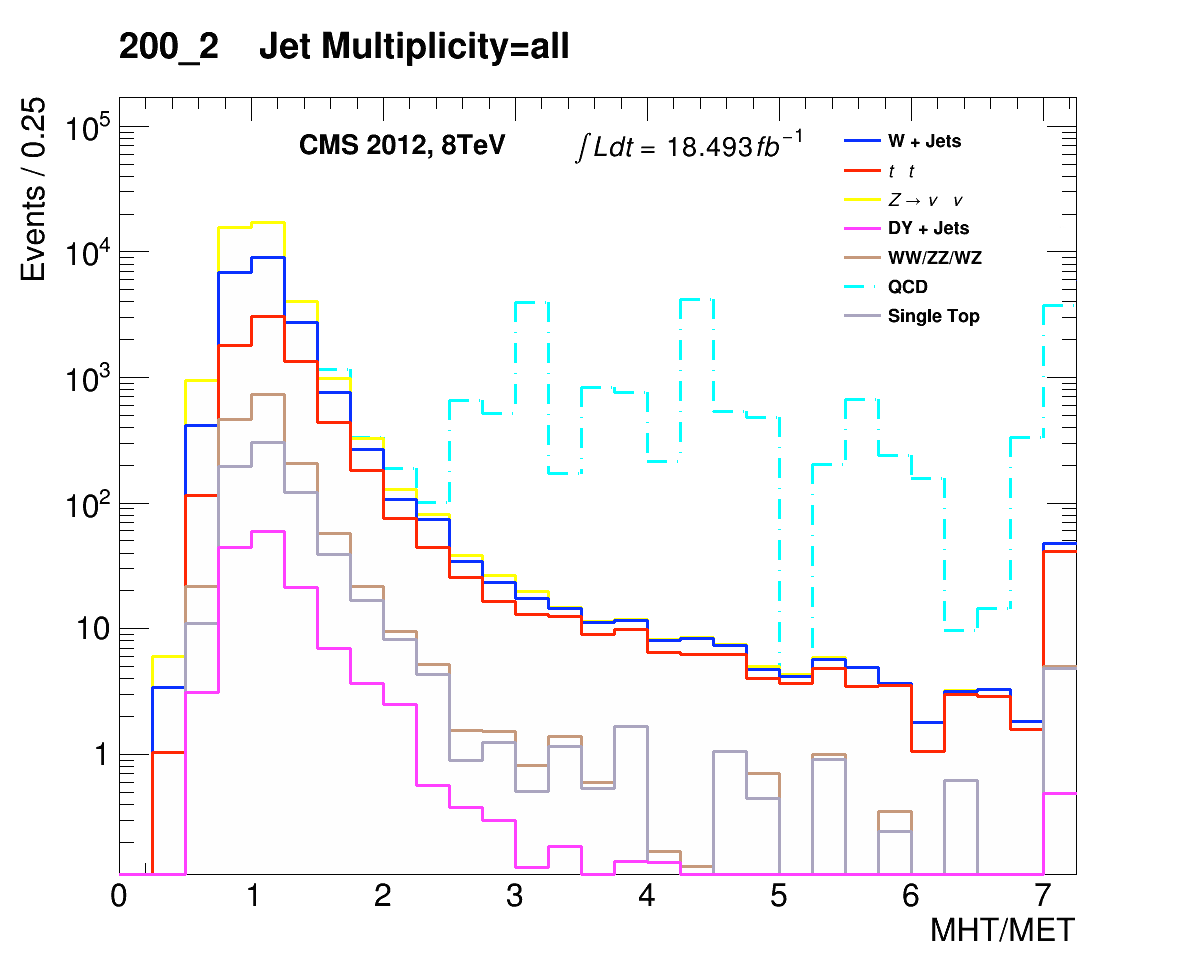
\includegraphics[width=0.6\textwidth]
{Figs/datamc/had/v1/Stacked_MHTovMET_all_200_upwards.png}
\caption{The \mhtmet distribution of MC events following the hadronic selection
criteria, minus the nominal \mhtmet requirement.The MC yields are stacked,
with the QCD contribution shown in cyan. The plot is for a fully inclusive
selection of $\nb \geq 0$, $\nj \geq 2$ and \HT > 200~\gev.}
\label{fig:full_mhtmet_distro}
\end{figure}

Events are able to acquire non-negligible amounts of \mht without the presence
of
real \met if multiple jets are below the jet \Pt threshold and their
configuration conspires to form a topology that gives high values of \alphat.
Such events will contain a disparity between the \met and
\mht variables, given that the former is reconstructed using energy deposits
and the latter with reconstructed jet objects.
Figure~\ref{fig:full_mhtmet_distro} shows the significant contribution of QCD at
high \mhtmet values, even following the \alphat requirement.
To protect against this scenario, events are required to have \mhtmet < 1.25.


\subsection{Instrumental effects}

Fake \mht may also be produced if jets overlap with areas of the calorimeter 
system which are damaged or known to be faulty (hereby referred to as `dead'),
and jets are mismeasured or lost as a result. To protect against this, for a
given jet $j$ the angular separation between the event \mht, calculated
excluding jet $j$, and the jet itself is defined as:
% 
\begin{equation}
\dphistar_j = \Delta \phi\big(\overrightarrow{\Pt}_j,-\sum_{i\neq j}
{\overrightarrow{\Pt}_i}\big) .
\label{eq:biasdphi}
\end{equation}
% 
An advantage of this variable with respect to the often used
$\Delta R(\overrightarrow{\Pt}_j, \mht)$ is it's detection of spurious missing
energy vectors
caused
by both under-measurements and over-measurements of a jet's energy.
A small value of $\dphistar_j$ indicates that the momentum vector of the jet $j$
is aligned with the \mht vector, implying the jet to be mismeasured. Events are
vetoed if a jet with \dphistar< 0.5 is within $\Delta R < 0.3$ of a known
`dead' region of the calorimeter.

To protect against further jet mismeasurements arising due to
instrumental effects, multiple event filters are applied. However, previously
undiscovered and therefore rare detector effects may still be
present. To check for such issues the
jet giving the minimum \dphistar value in an event, \mindphistar, is found
and a single entry of the $\eta$ and $\phi$ direction of the jet's axis is entered
into a map of the detector, shown in figure~\ref{fig:hotspots}. Any areas of
instrumental issue would
be visible as clusters of high event counts.
Figures~\ref{fig:hotspots_2d_nodeadECAL} and \ref{fig:hotspots_1d_nodeadECAL}
show the detector map and the 1D distribution
of counts before the dead ECAL filter is applied, with areas of
potential instrumental defects clearly visible, notably as outliers in
1D distribution. Following the application of the dead
ECAL filter the hotspot areas and the corresponding outliers are removed, as
seen in figures~\ref{fig:hotspots_2d_withdeadECAL} and
\ref{fig:hotspots_1d_withdeadECAL}. The lack of localised high-count regions or
the presence of a tail in the 1D distribution indicate there to be
no significant instrumental issues remaining.

\begin{figure}[h!]
  \begin{center}
    \begin{subfigure}[b]{0.46\textwidth}
      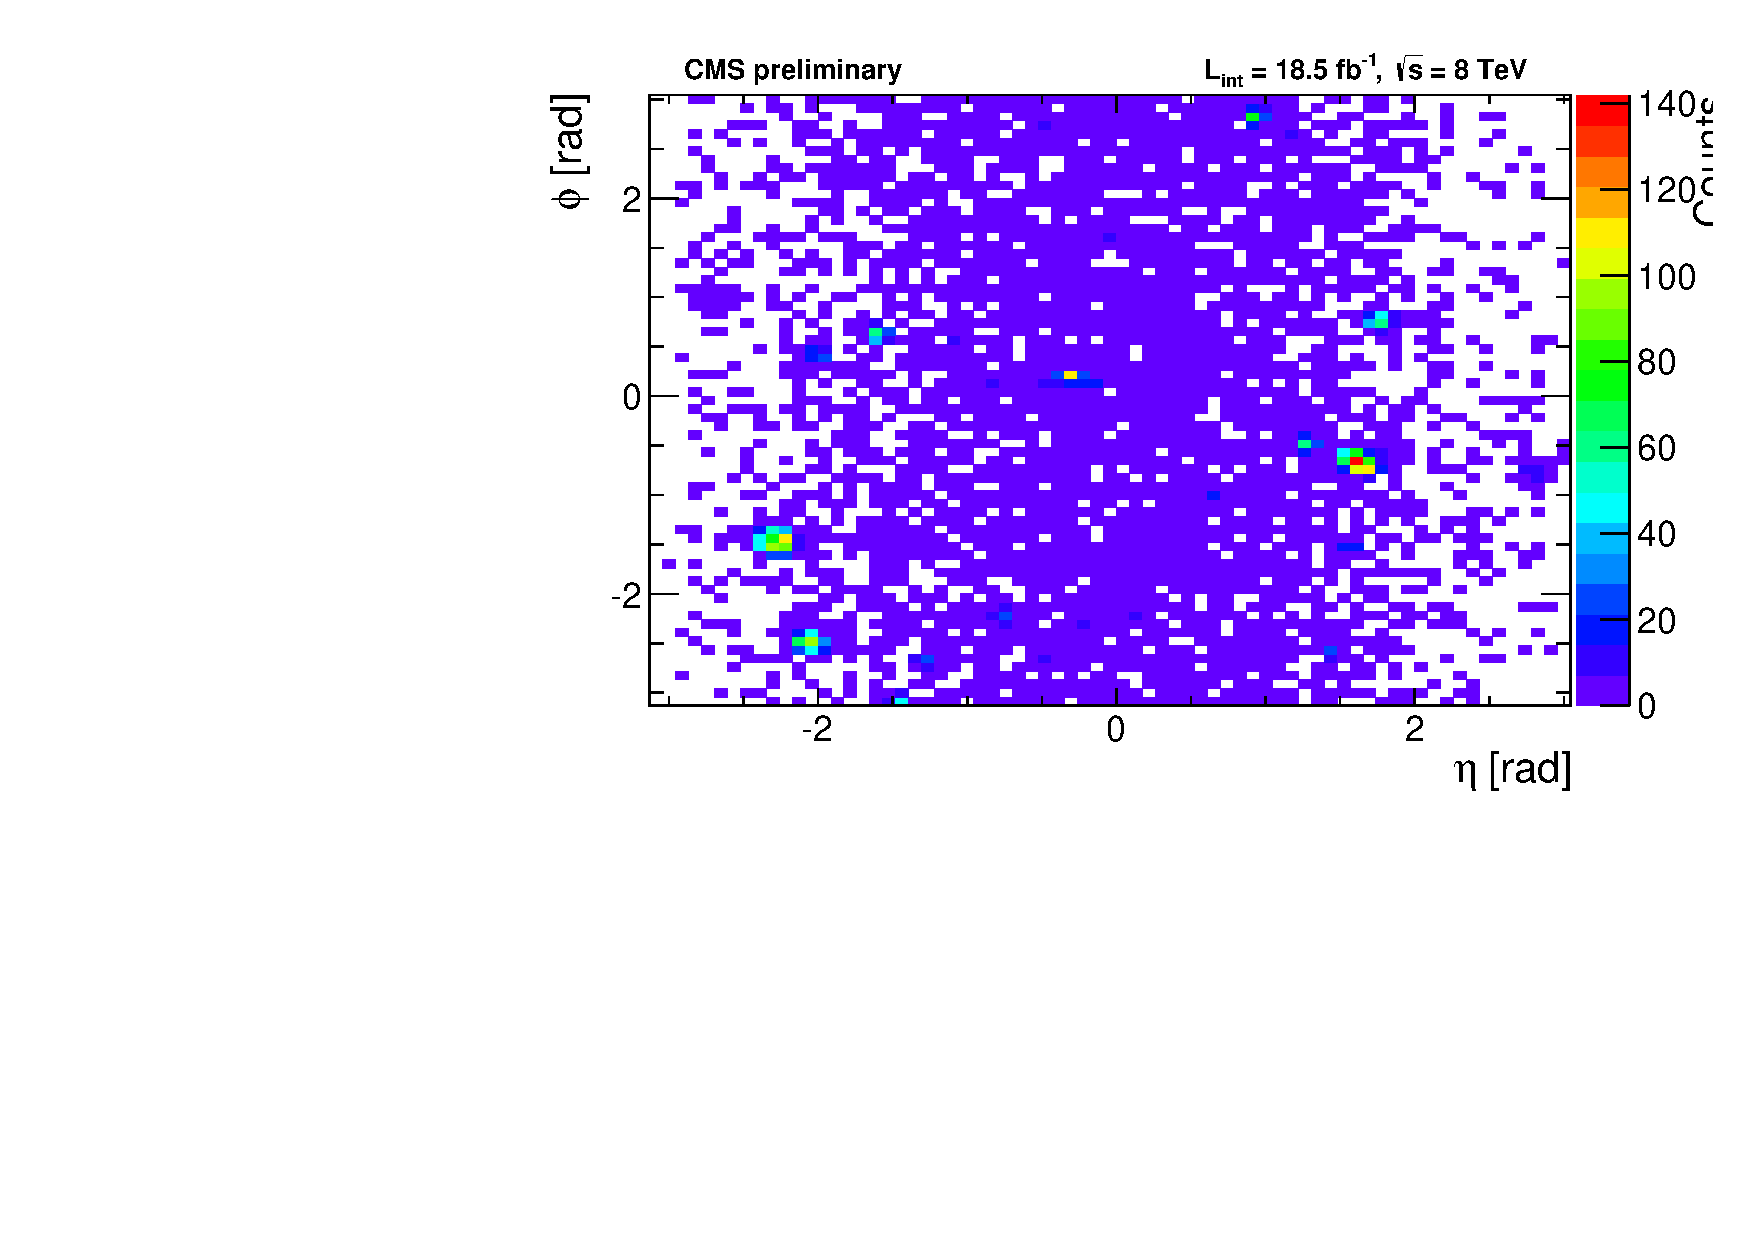
\includegraphics[width=\textwidth]{Figs/dphi/HT_dependent_AlphaT_thresholds/th2d_denom_summed_ge2j_ge0b_200.pdf}
      \caption{No ``dead ECAL filter''.}
      \label{fig:hotspots_2d_nodeadECAL}
    \end{subfigure}
    \begin{subfigure}[b]{0.46\textwidth}
      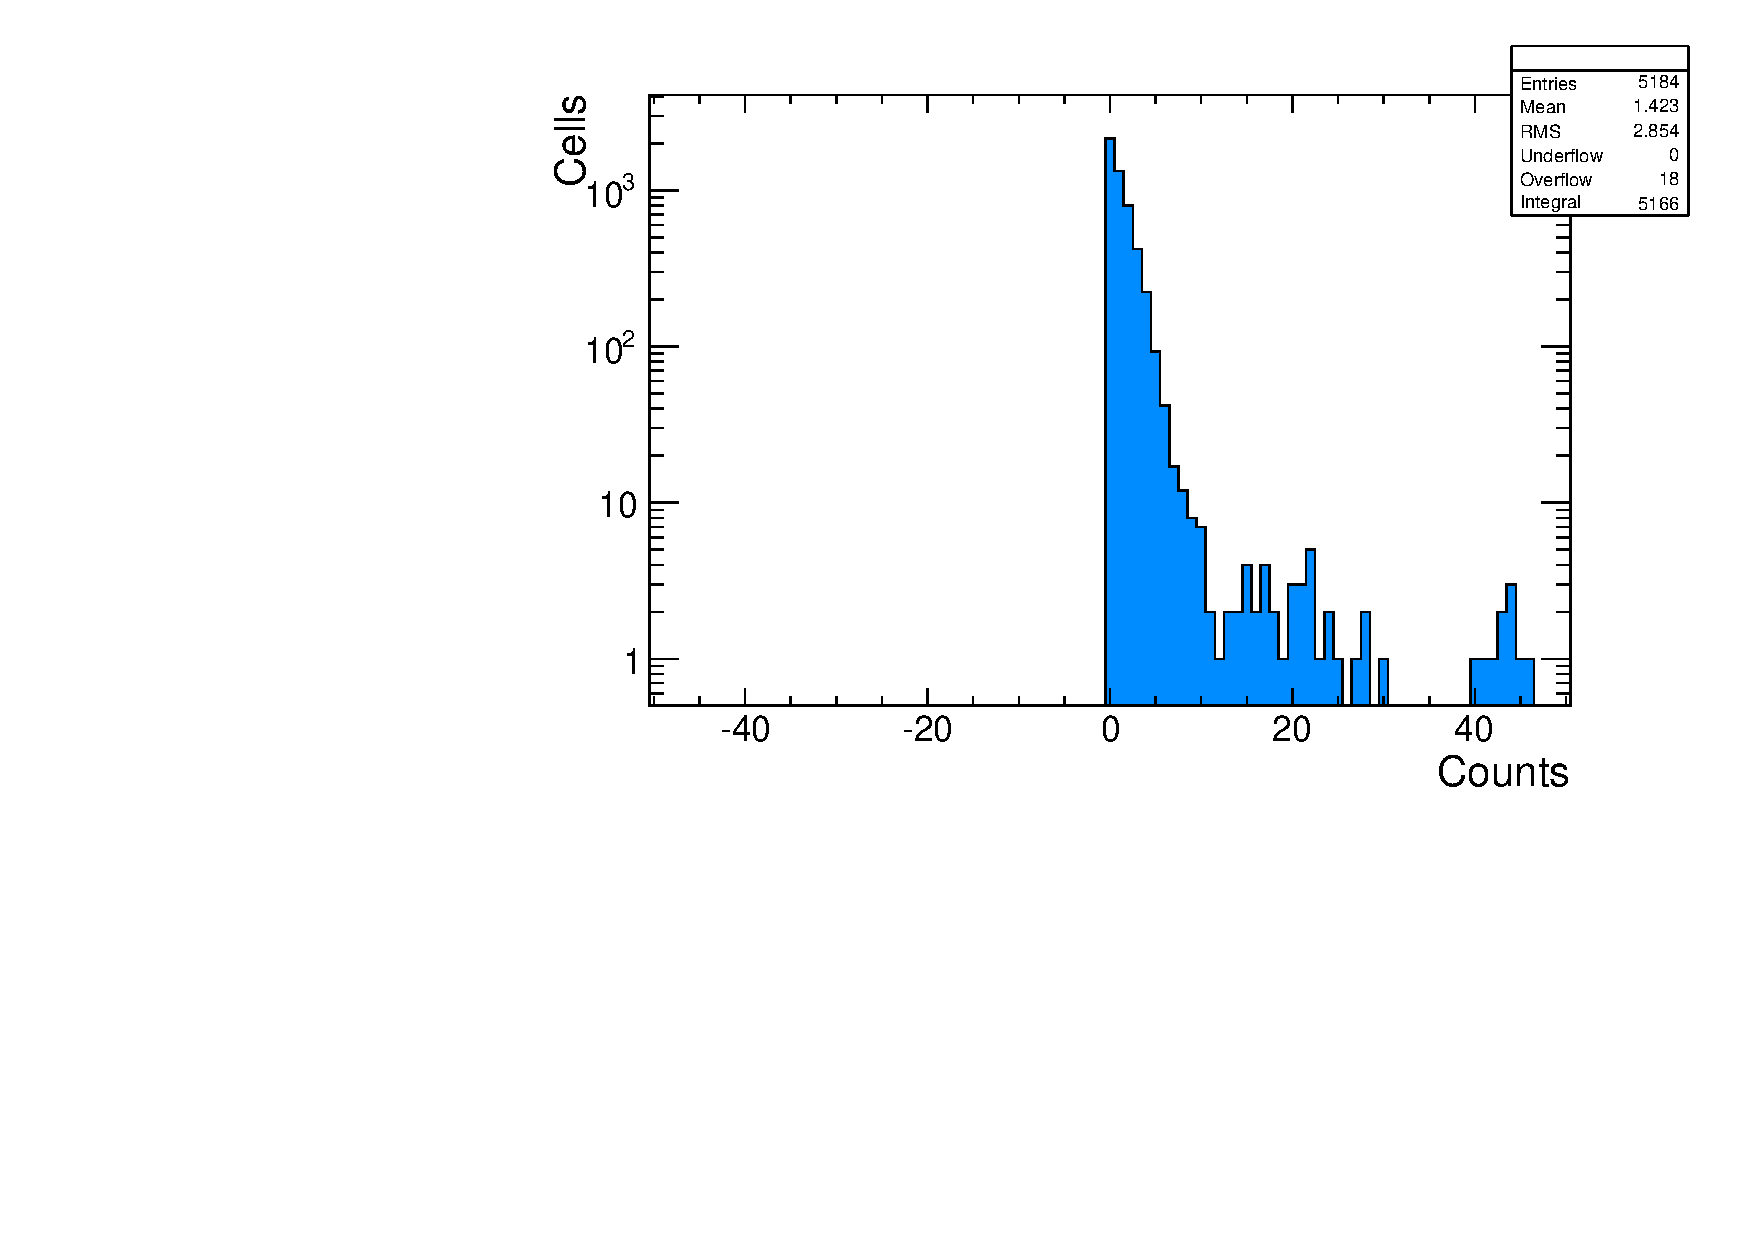
\includegraphics[width=\textwidth]{Figs/dphi/HT_dependent_AlphaT_thresholds/th1d_denom_summed_ge2j_ge0b_200.pdf}
      \caption{No ``dead ECAL filter''.}
      \label{fig:hotspots_1d_nodeadECAL}
    \end{subfigure} \\ 
    \begin{subfigure}[b]{0.46\textwidth}
      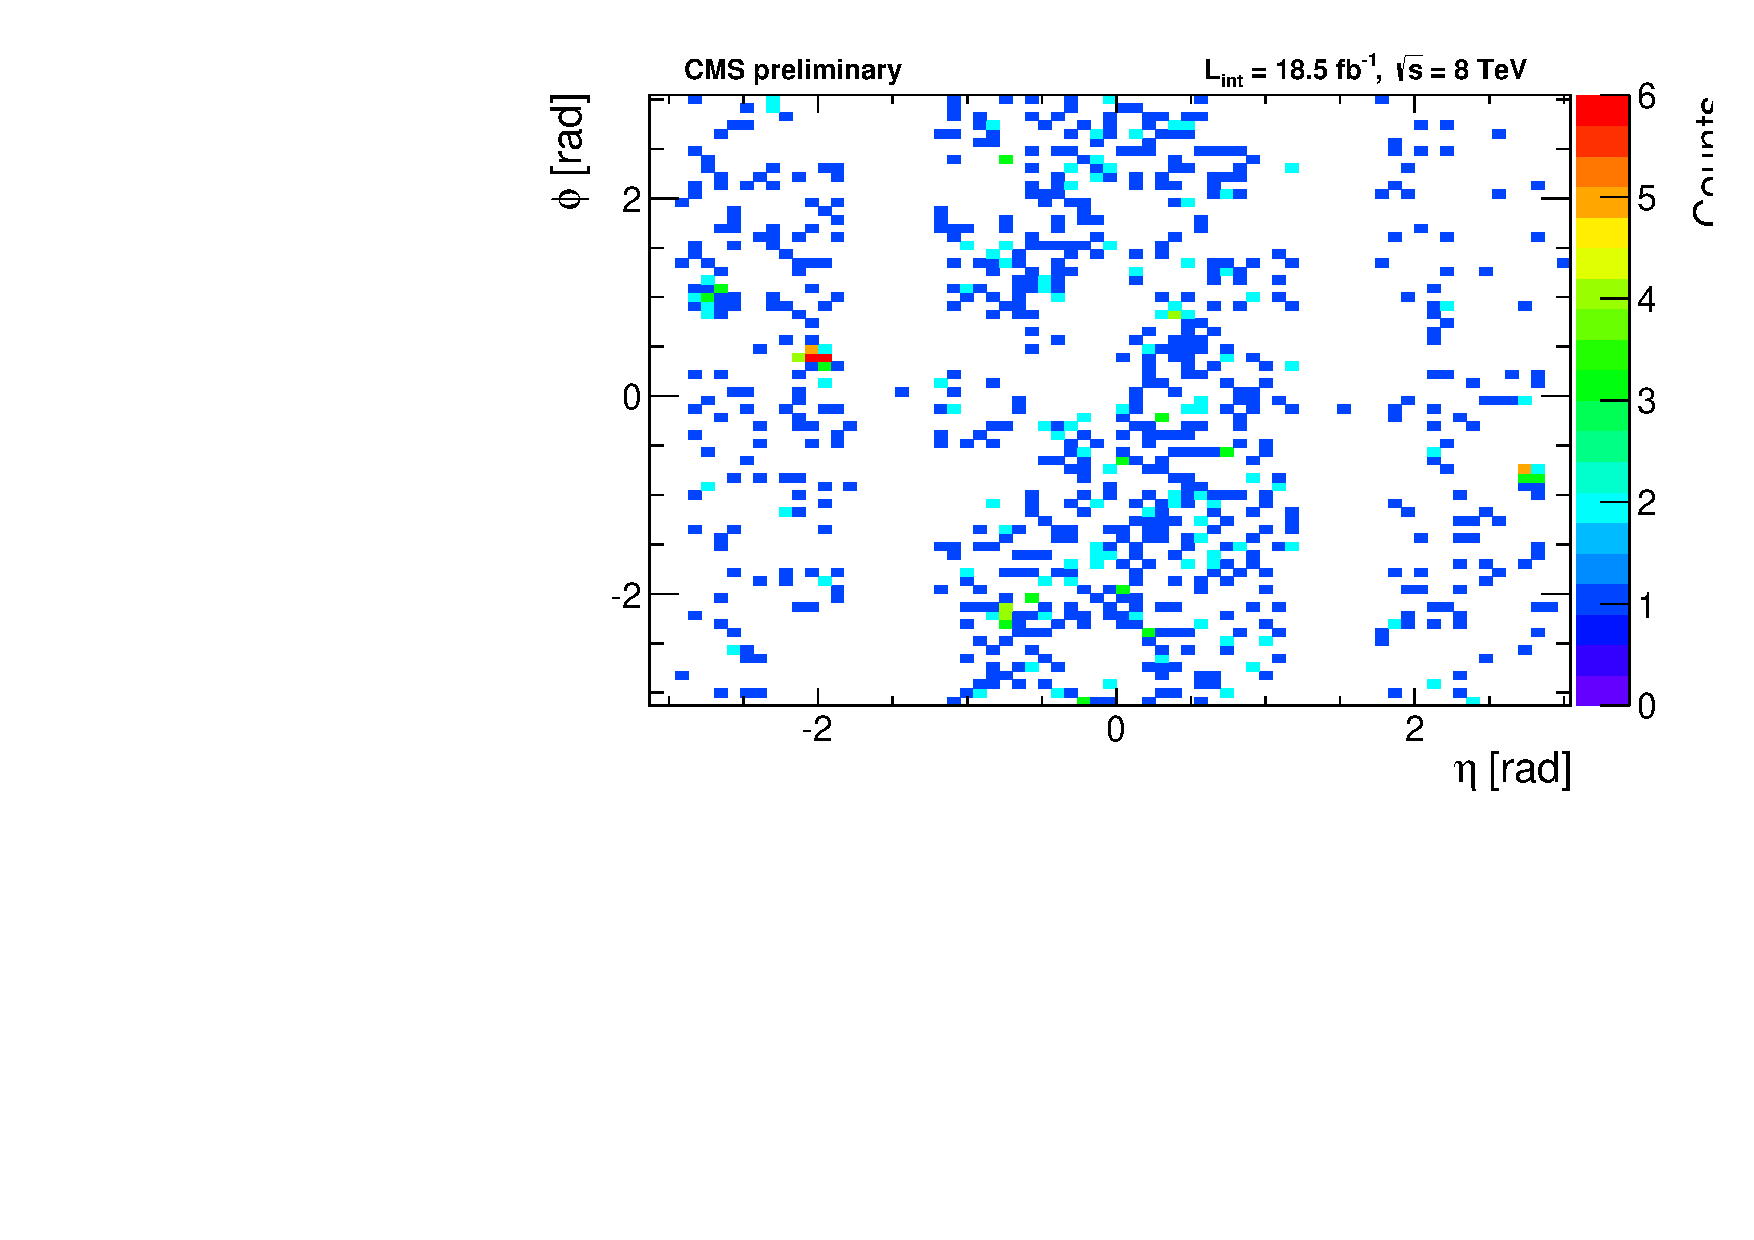
\includegraphics[width=\textwidth]{Figs/dphi/Nominal_AlphaT_thresholds/th2d_numer_summed_ge2j_ge0b_200.pdf}
      \caption{With ``dead ECAL filter''.}
      \label{fig:hotspots_2d_withdeadECAL}
    \end{subfigure}
    \begin{subfigure}[b]{0.46\textwidth}
      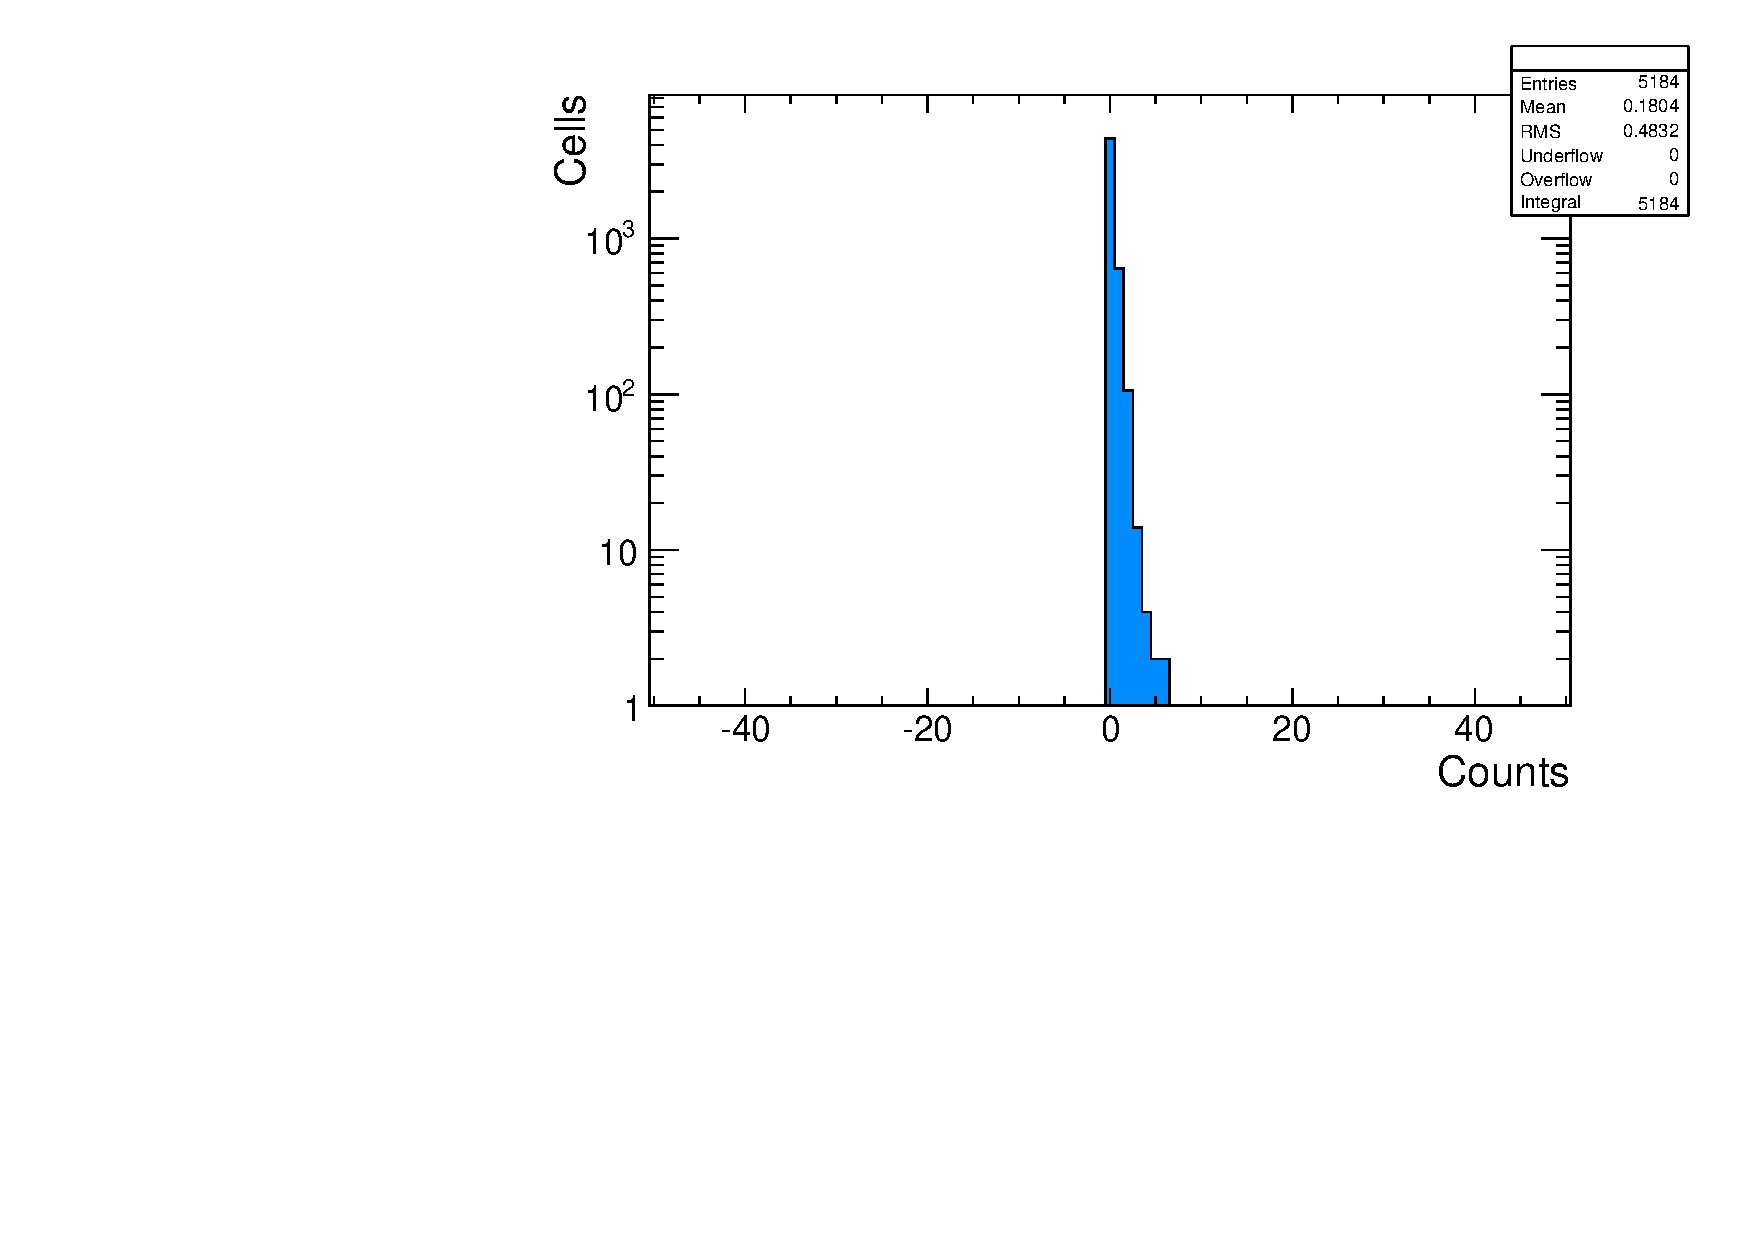
\includegraphics[width=\textwidth]{Figs/dphi/Nominal_AlphaT_thresholds/th1d_numer_summed_ge2j_ge0b_200.pdf}
      \caption{With ``dead ECAL filter''.}
      \label{fig:hotspots_1d_withdeadECAL}
    \end{subfigure} \\ 
    \caption{Distribution of jets in ($\eta$, $\phi$)-space that are
      responsible for an event satisfying the requirement $\mindphistar <
      0.3$, with (a, b) and without (c, d) the ``dead ECAL filter''
      requirement applied as part of the signal region selection.}
    \label{fig:hotspots}
  \end{center}
\end{figure}

\subsection{Heavy-flavour jet decays}

Jets can also appear to be mismeasured if the parton
shower contains heavy flavour mesons which decay leptonically EXAMPLE. In rare
circumstances, these decays can give the largest fraction of the available
momenta to the neutrino, leading to significant amounts of real \met and
soft-leptons which can evade the lepton vetoes.
This effect is compounded when multiple neutrinos are produced in the shower,
with a significant fraction of the jet's energy therefore evading detection. An
example event display is shown in appendix~\ref{ch:app_dphistar}, in
figure~\ref{fig:event_display_QCD}.

To better study events of this type a study region is defined, populated by the
the single-object \HT trigger, \verb!HLT_HT750!, which remained unprescaled
throughout \runone. As opposed to a typical signal trigger, the lack of an
\alphat requirement allows lower regions of \alphat to be studied. The region is
therefore defined by \HT > 775~\gev and \alphat > 0.507, where this trigger is
fully efficient. Due to the intrinsic correlation of \HT and \mht within the
\alphat variable (figure~\ref{fig:alphat_mht_corr}), this selection provides
an effective \mht requirement similar to that of the low \HT categories of the
nominal analysis.

\begin{figure}[b!]
  \centering
  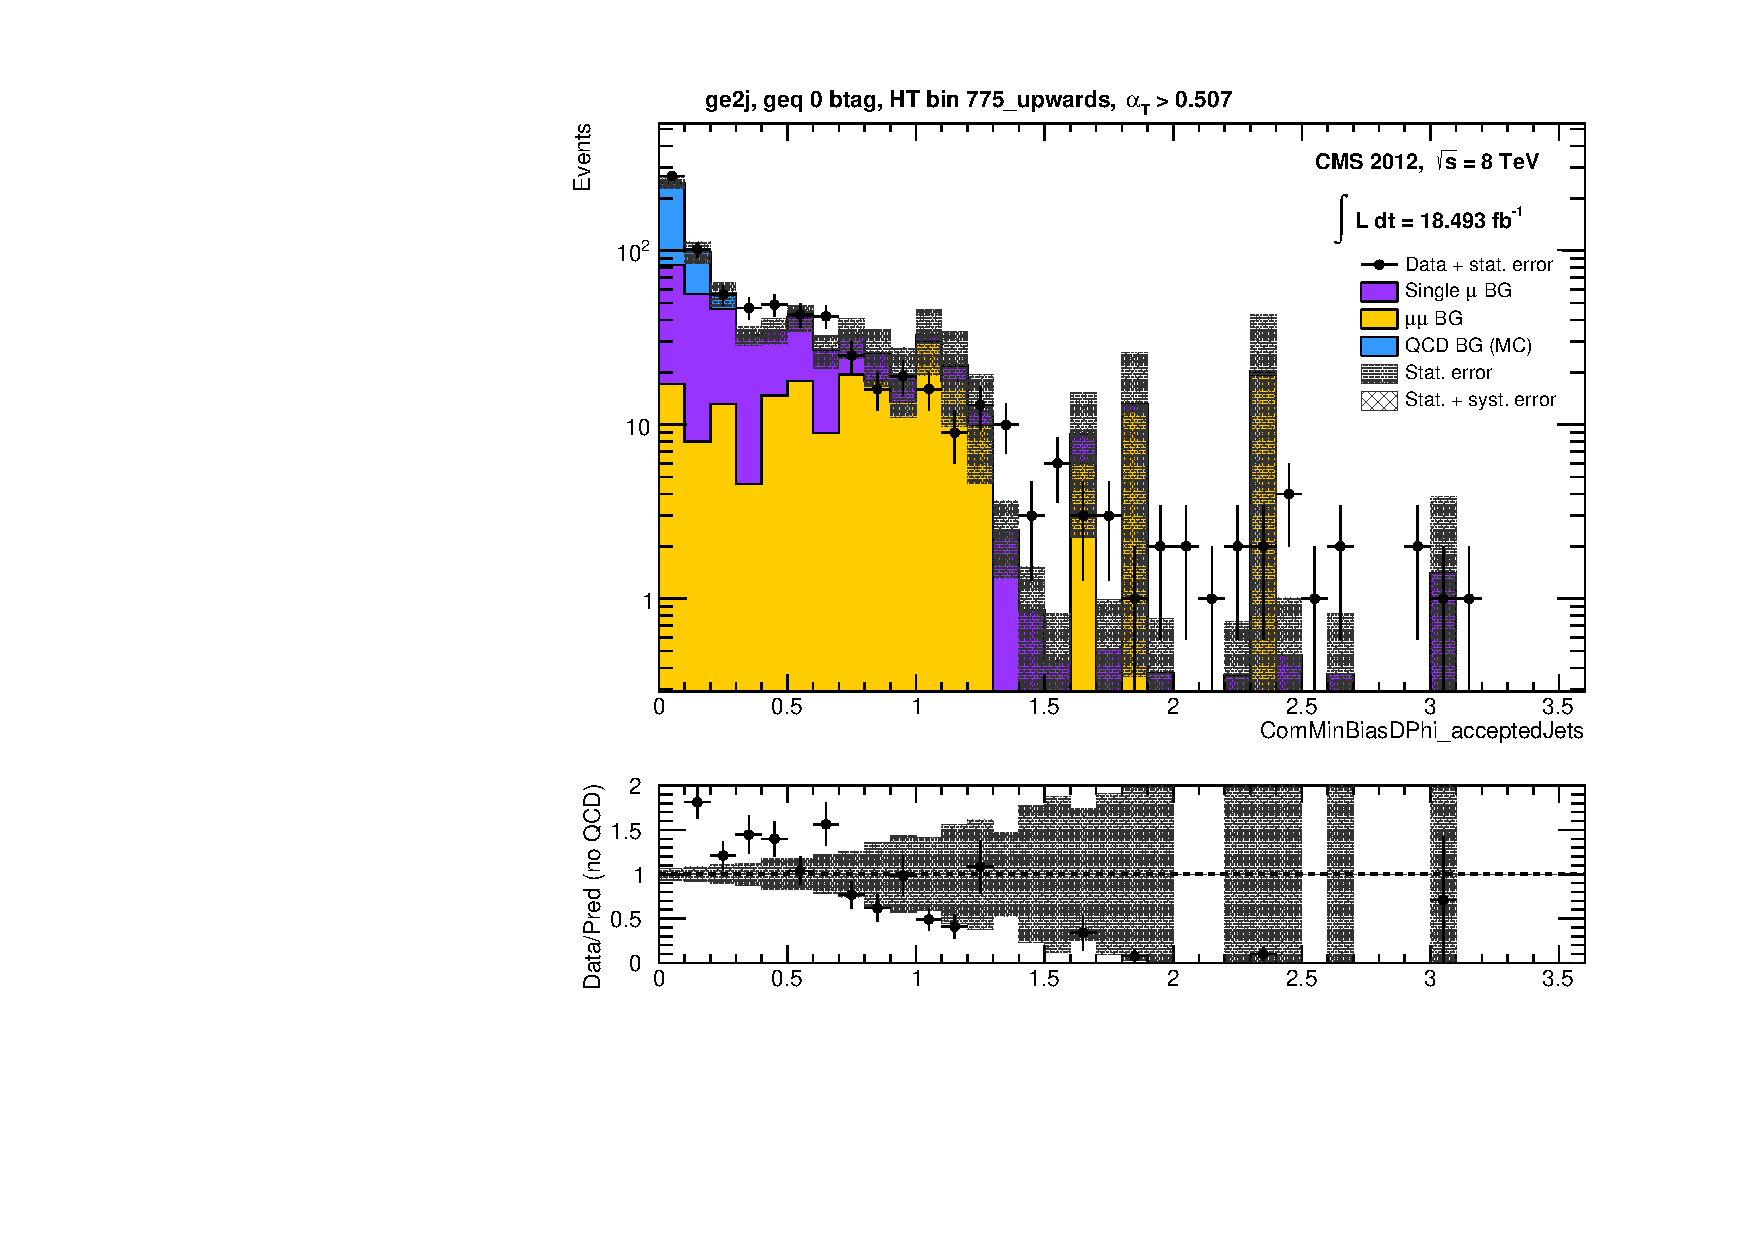
\includegraphics[width=0.6\textwidth]
  {Figs/datapred/qcd_study_region/ge2j_ge0b_775_upwards/Prediction_ComMinBiasDPhi_acceptedJets_all_775_upwards_QCD}
  \caption{Data (black points) against the EWK background prediction 
  (stacked, yellow and purple) as a function of \mindphistar. The expected yield
  from QCD MC (cyan) is stacked on top of the EWK prediction, but not included
  in the ratio plot. The plot represents
  the QCD control study region, with $\nb \geq 0$, $\nj \geq 2$, $\HT > 775
 ~\gev$ and $\alphat > 0.507$.}
  \label{fig:qcd_region_pred_dphistar_incl}
\end{figure}

Jets containing a \met source will appear as mismeasured and therefore
populate a region of low \dphistar (equation~\ref{eq:biasdphi}).
Figure~\ref{fig:qcd_region_pred_dphistar_incl} shows the data compared to the
EWK background prediction (this method is discussed later in
chapter~\ref{ch:background})
as a function of the \mindphistar value of each event. The disagreement observed
at low \mindphistar is well accounted for by the yield from QCD MC. However, it
should be noted that while MC can provide a qualitative understanding of the QCD
contamination, it should not be relied upon to determine a quantitative
understanding of the phenomenon.

As motivated by figure~\ref{fig:qcd_region_pred_dphistar_incl}, the residual QCD
events appear to be well isolated in the region $\mindphistar < 0.3$. The effect
of applying this threshold in the QCD control study region is shown in
figure~\ref{fig:data_pred_dphistar_eff}.
% 
\begin{figure}[h!]
  \centering
  \begin{subfigure}[b]{0.46\textwidth}
    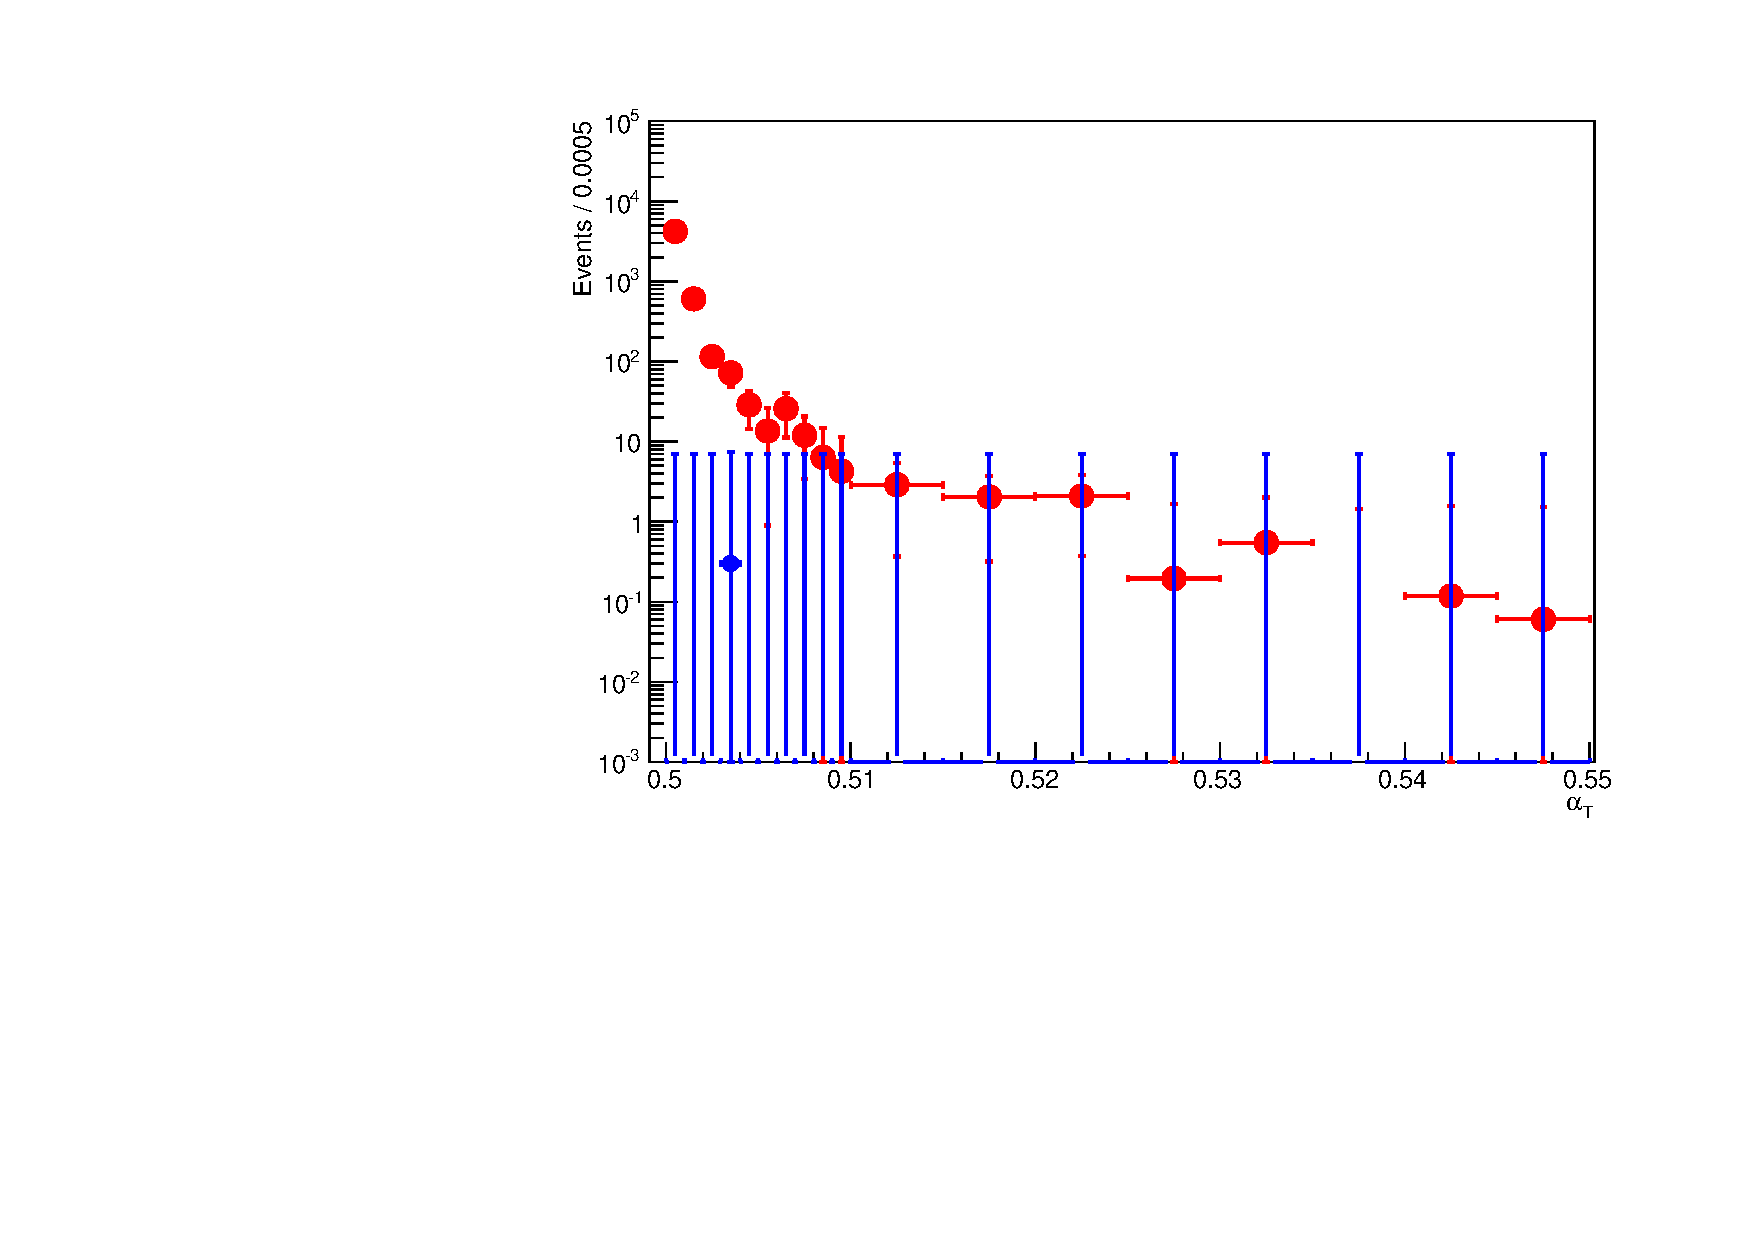
\includegraphics[width=\textwidth]{Figs/dphi/chris2/qcd_mc/dphi_incl/v2/dphi_eq3j_ge0b_775}
    \caption{$\nj = 3$, simulation}
    \label{fig:dphi_acceptance_sim_3j}
  \end{subfigure}
  \begin{subfigure}[b]{0.46\textwidth}
    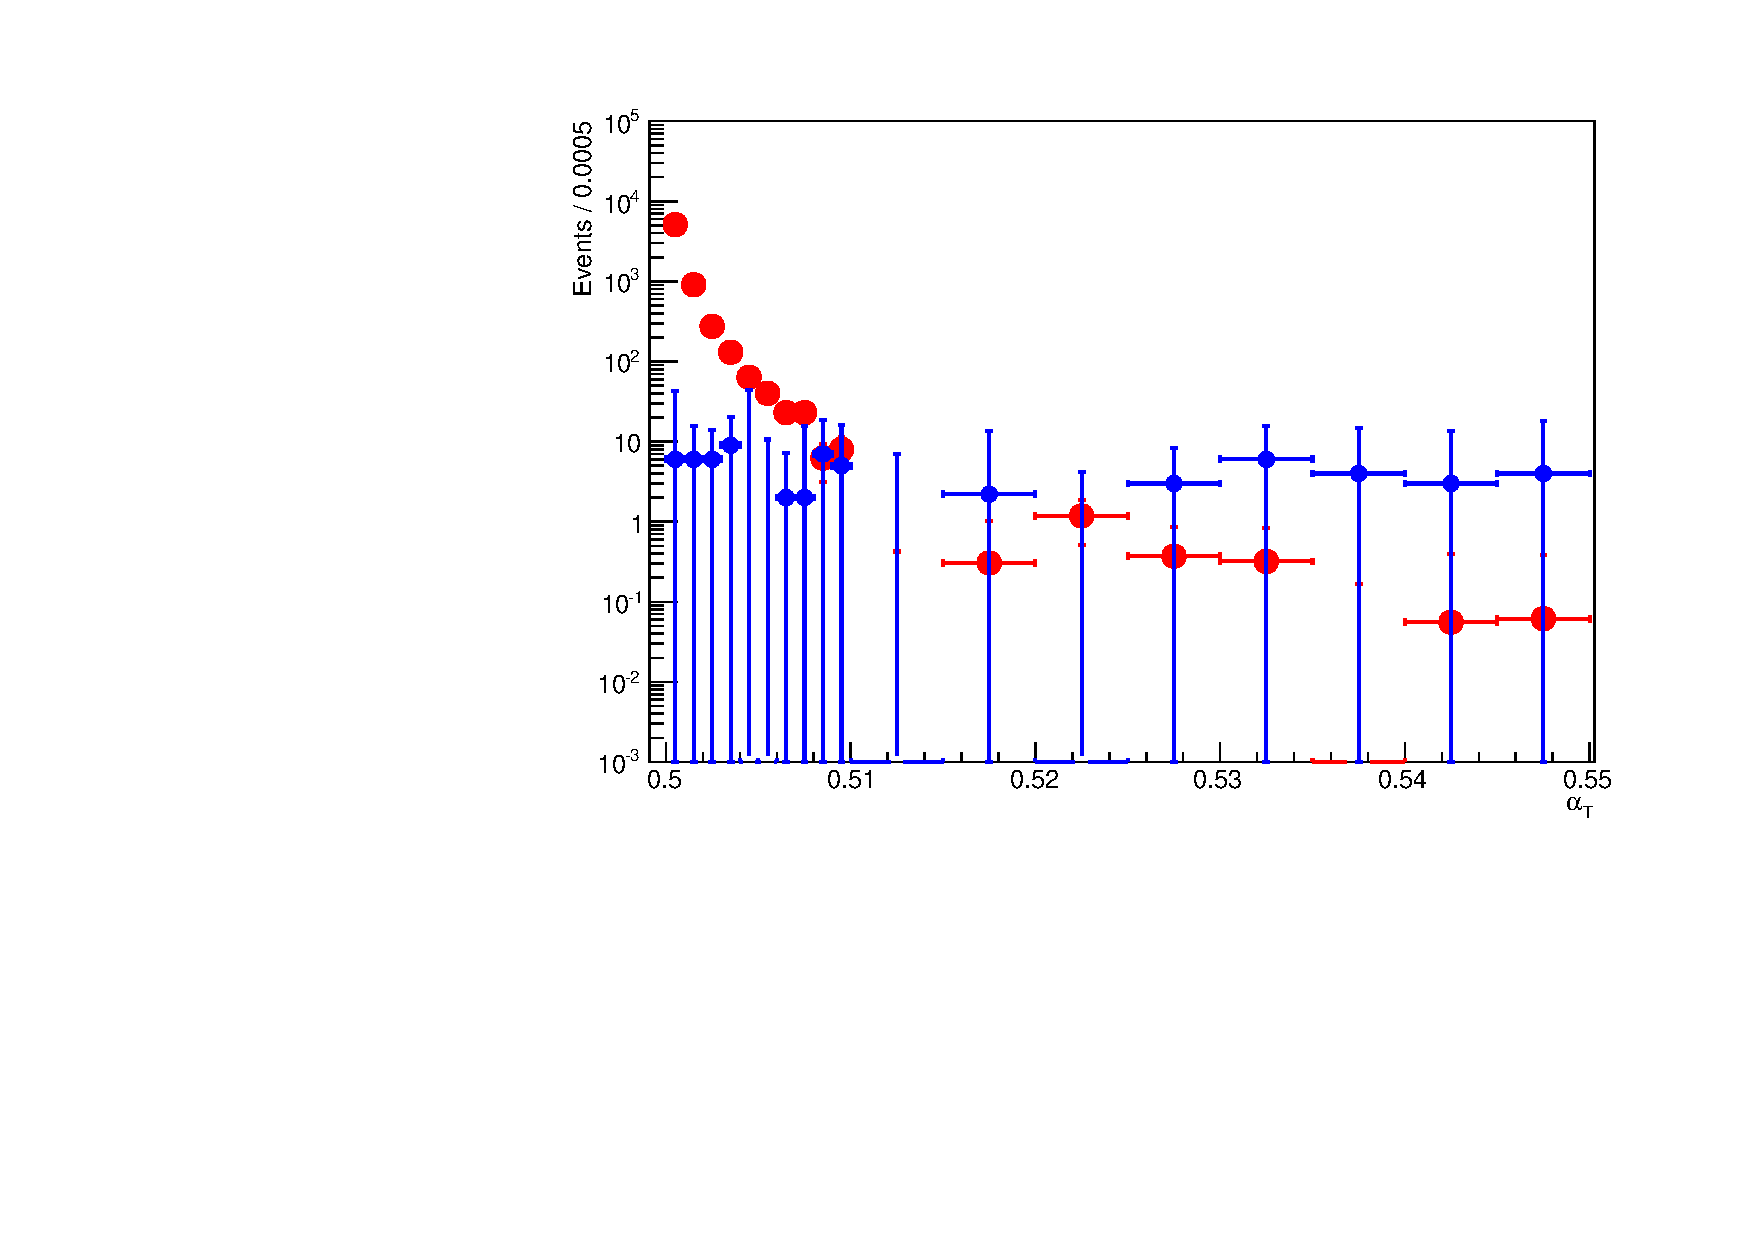
\includegraphics[width=\textwidth]{Figs/dphi/chris2/data/dphi_incl/v2/dphi_eq3j_ge0b_775}
    \caption{$\nj = 3$, data}
    \label{fig:dphi_acceptance_data_3j}
  \end{subfigure}\\
  \begin{subfigure}[b]{0.46\textwidth}
    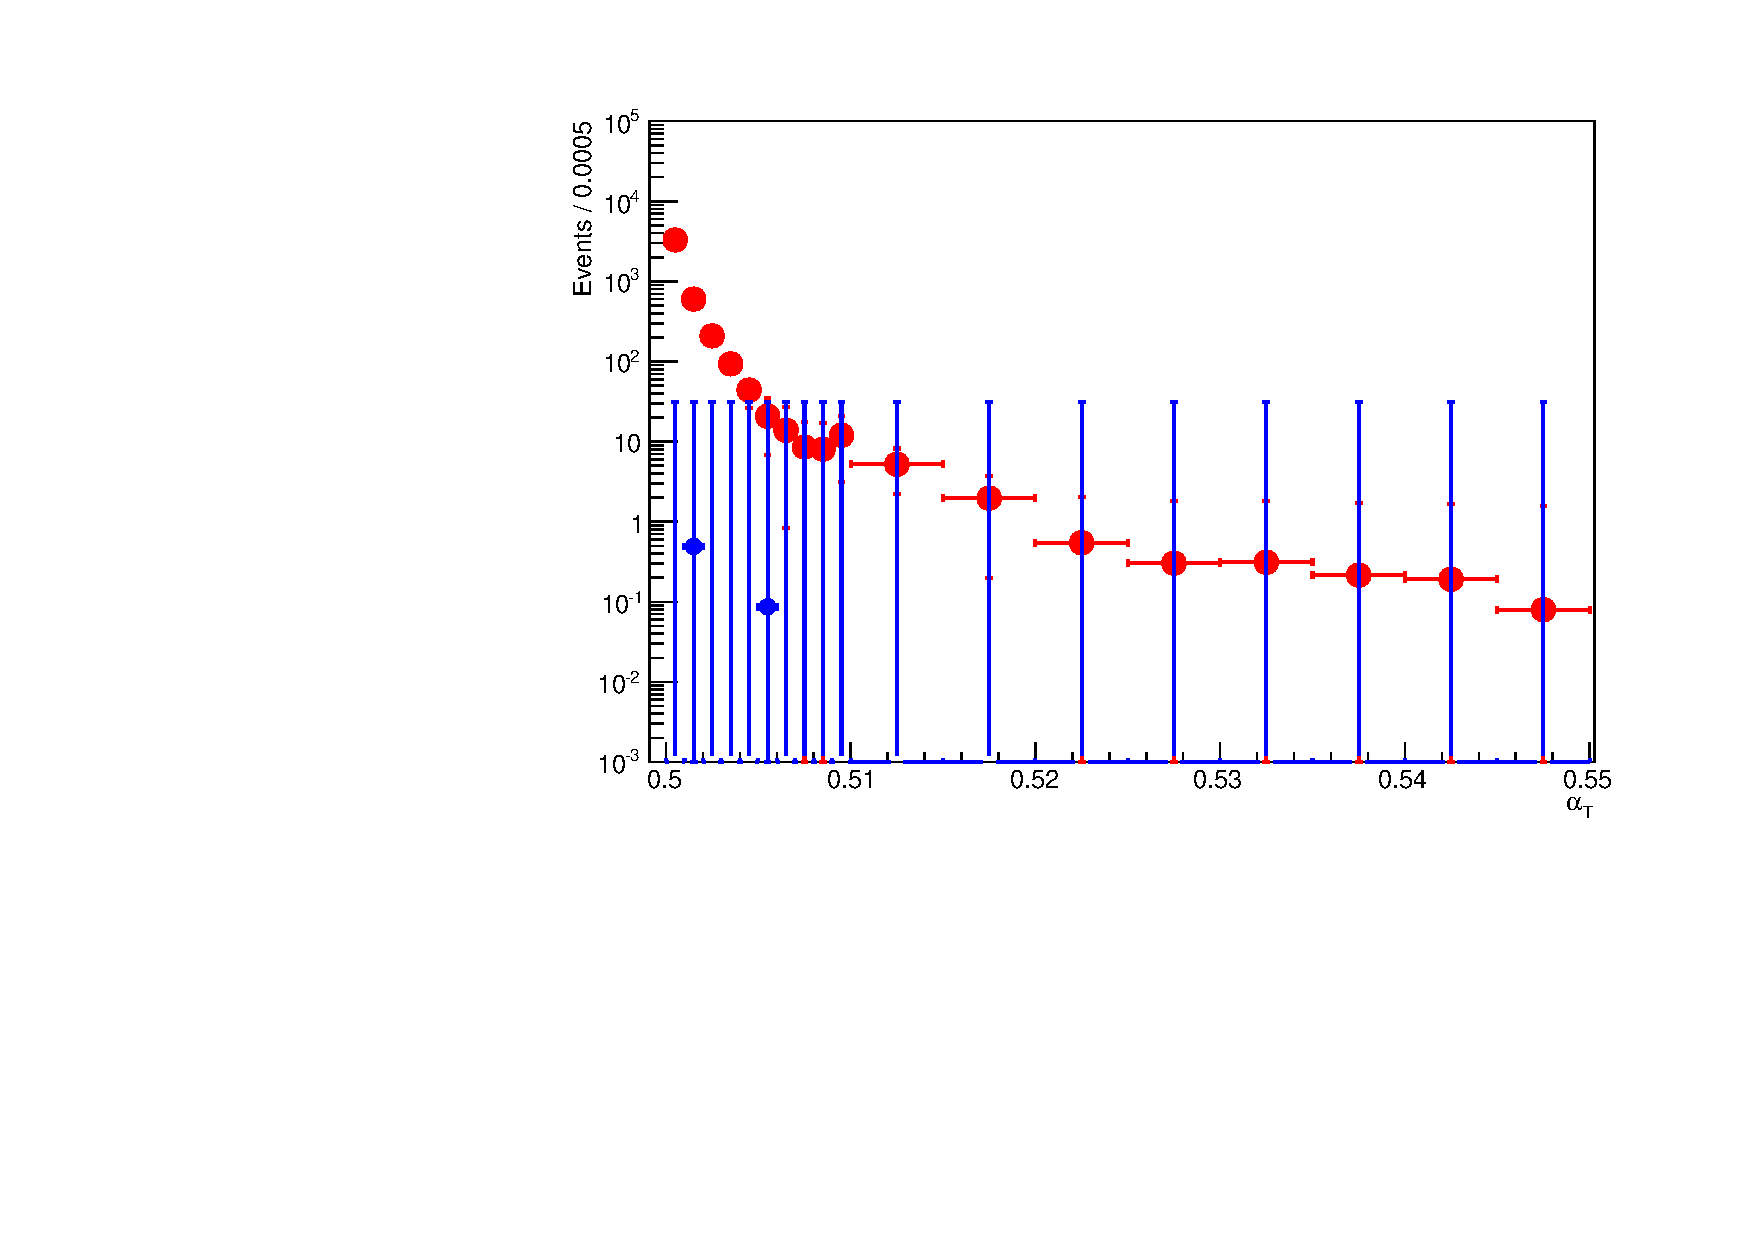
\includegraphics[width=\textwidth]{Figs/dphi/chris2/qcd_mc/dphi_incl/v2/dphi_eq4j_ge0b_775}
    \caption{$\nj = 4$, simulation}
    \label{fig:dphi_acceptance_sim_4j}
  \end{subfigure}
  \begin{subfigure}[b]{0.46\textwidth}
    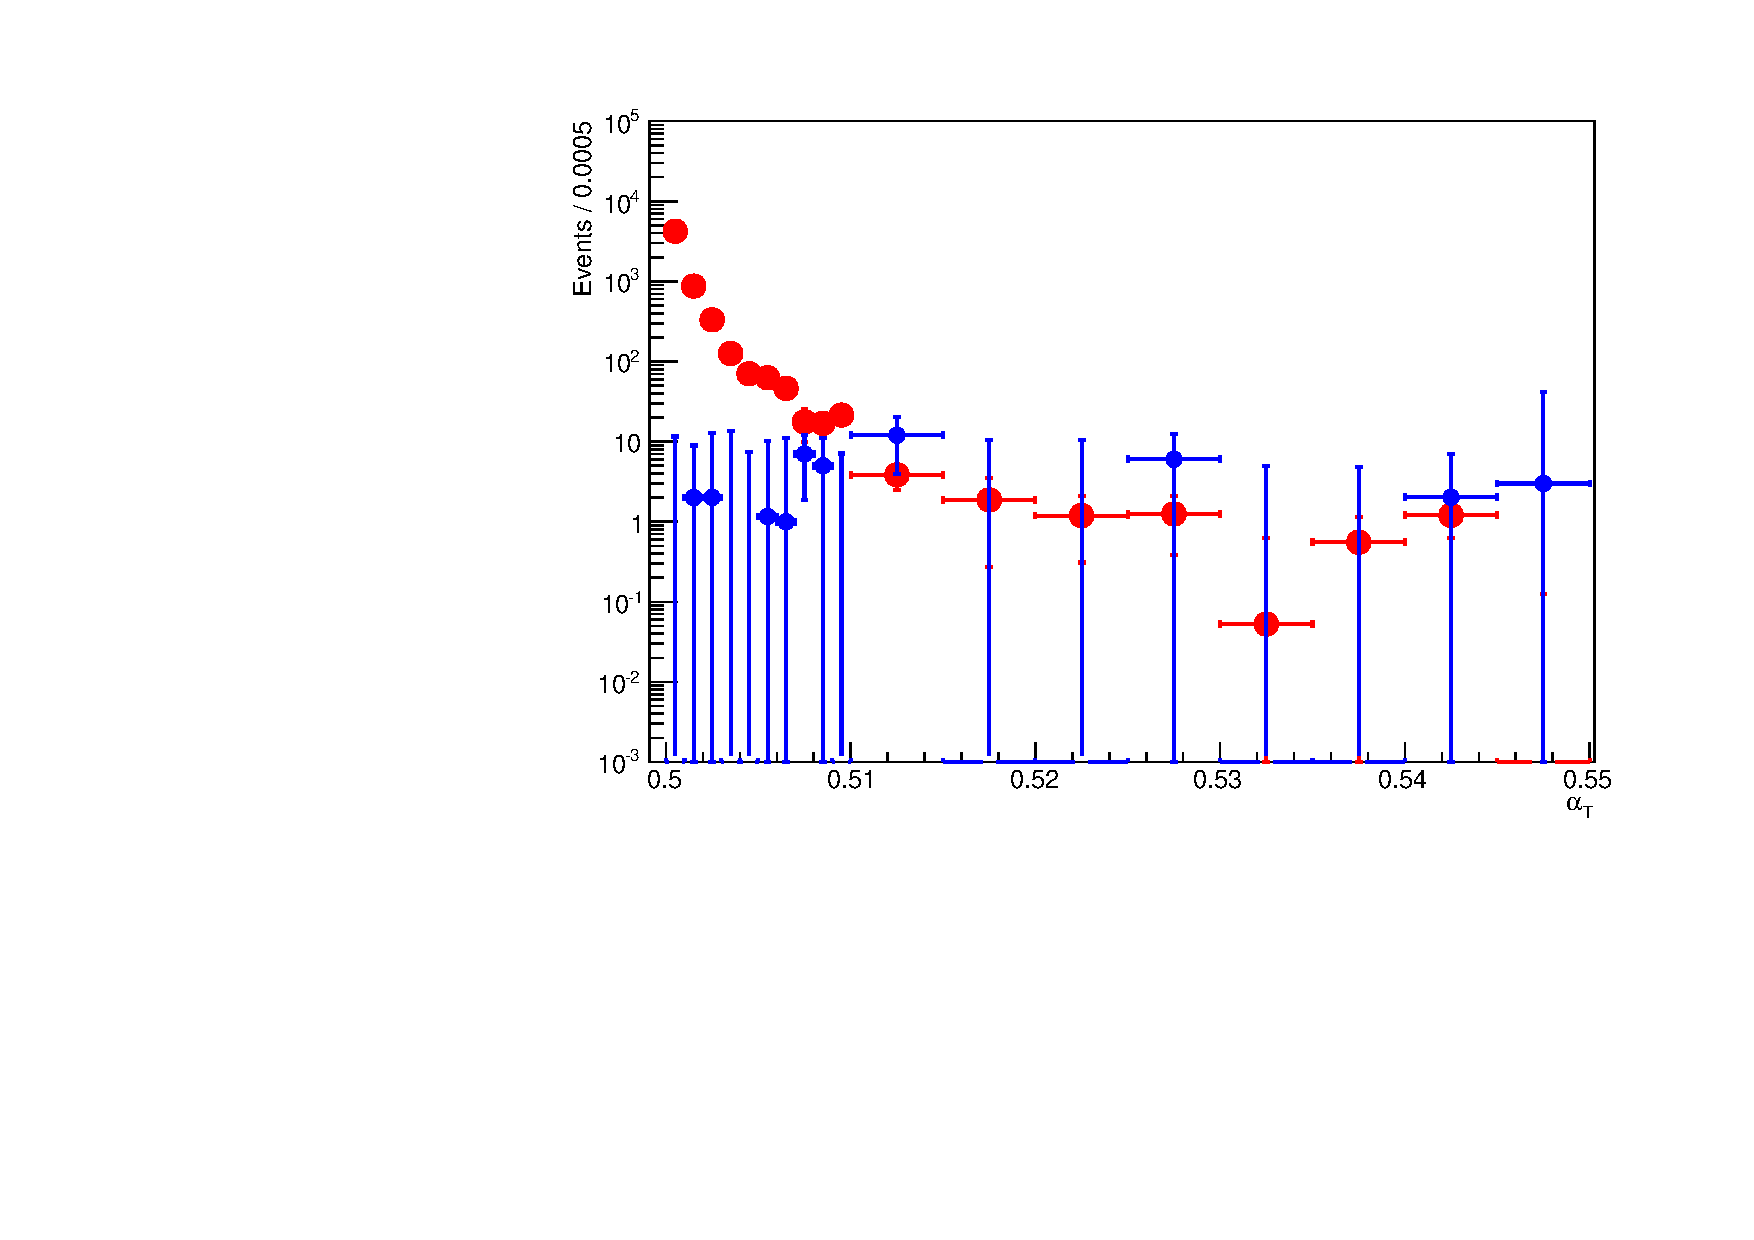
\includegraphics[width=\textwidth]{Figs/dphi/chris2/data/dphi_incl/v2/dphi_eq4j_ge0b_775}
    \caption{$\nj = 4$, data}
    \label{fig:dphi_acceptance_data_4j}
  \end{subfigure}\\
  \caption{The \alphat distribution for events with no \mindphistar
    requirement (red circles) and with the $\mindphistar > 0.3$
    requirement (blue circles) as determined from QCD multijet
    simulation (left column) or data (right column) and the exclusive
    $\nj =3$
    (top row) or $\nj = 4$ (bottom row). Note that negligible QCD contamination
    is seen in the $\nj = 2$ category, not shown here. The QCD control study
    region requirements have been applied, $\HT > 775$~\gev and $\alphat >
    0.507$, with $\nb \geq 0$.}
    \label{fig:data_pred_dphistar_eff}
\end{figure}
% 
When considering simulation (figures~\ref{fig:dphi_acceptance_sim_3j} and
\ref{fig:dphi_acceptance_sim_4j}), the requirement of \mindphistar > 0.3 appears
to remove any contributions particularly at high values of \alphat. However care
must be taken when interpreting the same plots for data
(figures~\ref{fig:dphi_acceptance_data_3j} and
\ref{fig:dphi_acceptance_data_4j}). To extract the QCD MJ contribution from
data,
observed event counts are corrected to subtract the contribution from the EWK
background processes, as estimated using the standard EWK background prediction
process which itself has inherent statistical and systematic uncertainties.
Subsequently, the QCD prediction as shown in the plots, has a non-zero error
associated
with it. Despite this, it is still visible that the \mindphistar > 0.3
requirement
leads to QCD MJ observations in data that are compatible with zero.

Events with jets containing real \met sources are likely to have
$\mht \approx \met$ by definition, and would therefore not be protected against
by the \mhtmet threshold
described in section~\ref{sec:qcd_cleaning_below_thresh}. Consider the ratio
of events passing and failing the \mhtmet requirement, as
% 
\begin{equation}
\label{eq:rmhtmet}
\rmhtmet = \frac{N(\mhtmet<1.25)}{N(\mhtmet>1.25)}.
\end{equation}
% 
Another method to determine the QCD MJ contamination is to study this variable
plotted as a function of \alphat after subtracting the
predicted EWK background, leaving only QCD multijet events.
In the absence of events with jets containing sources of real \met, a strong
exponential decrease as a function of \alphat would be expected. However, given
these events populate the
\mhtmet < 1.25 region, a constant pedestal in \alphat is observed, as is shown
in figure~\ref{fig:rmhtmet_dphi_data_sim}.

  \begin{figure}[p!]
    \centering
    \begin{subfigure}[b]{0.46\textwidth}
      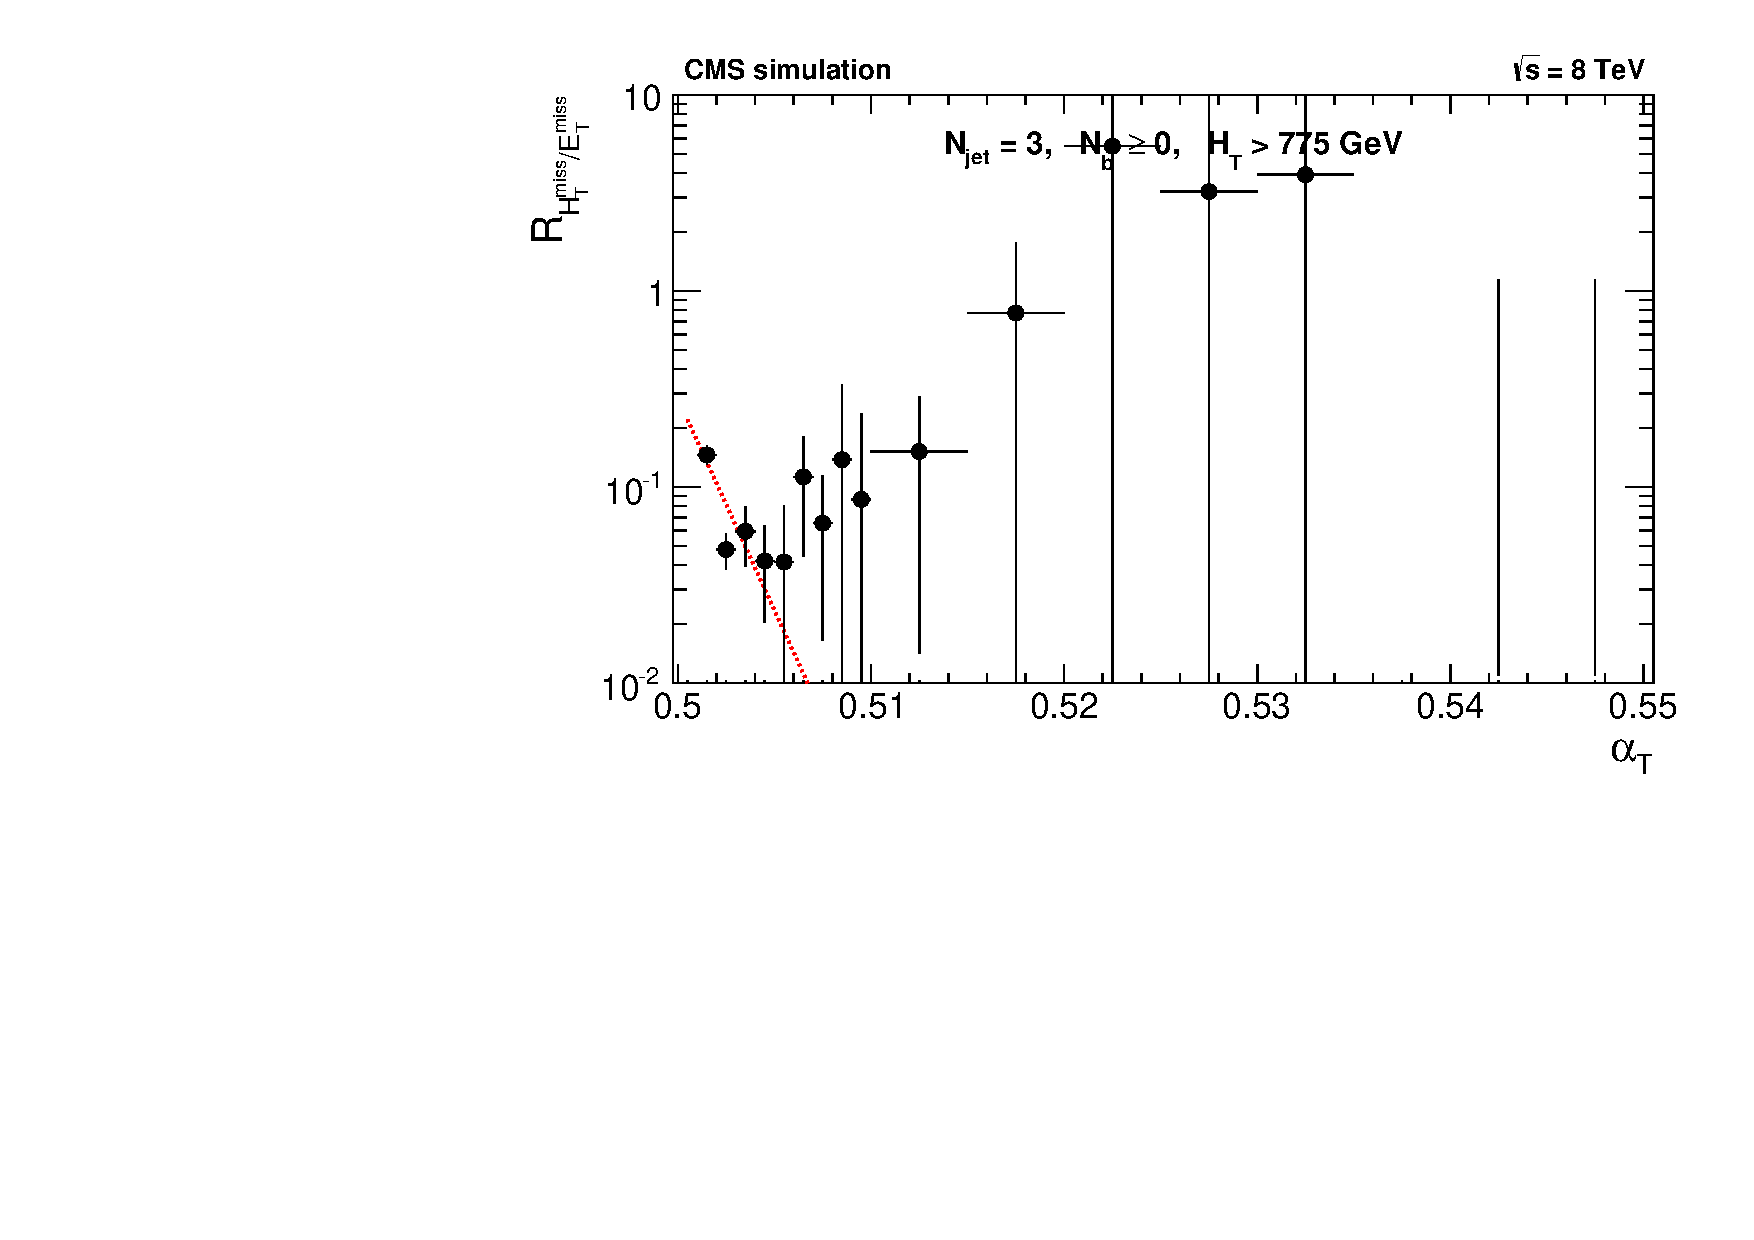
\includegraphics[width=\textwidth]{Figs/dphi/chris2/qcd_mc/dphi_lt0p3/v2/ratio_eq3j_ge0b_775}
      \caption{Simulation, $\nj = 3$, \mindphistar < 0.3}
      \label{fig:rdphi_sim_j3_lt0p3}
    \end{subfigure}
    \begin{subfigure}[b]{0.46\textwidth}
      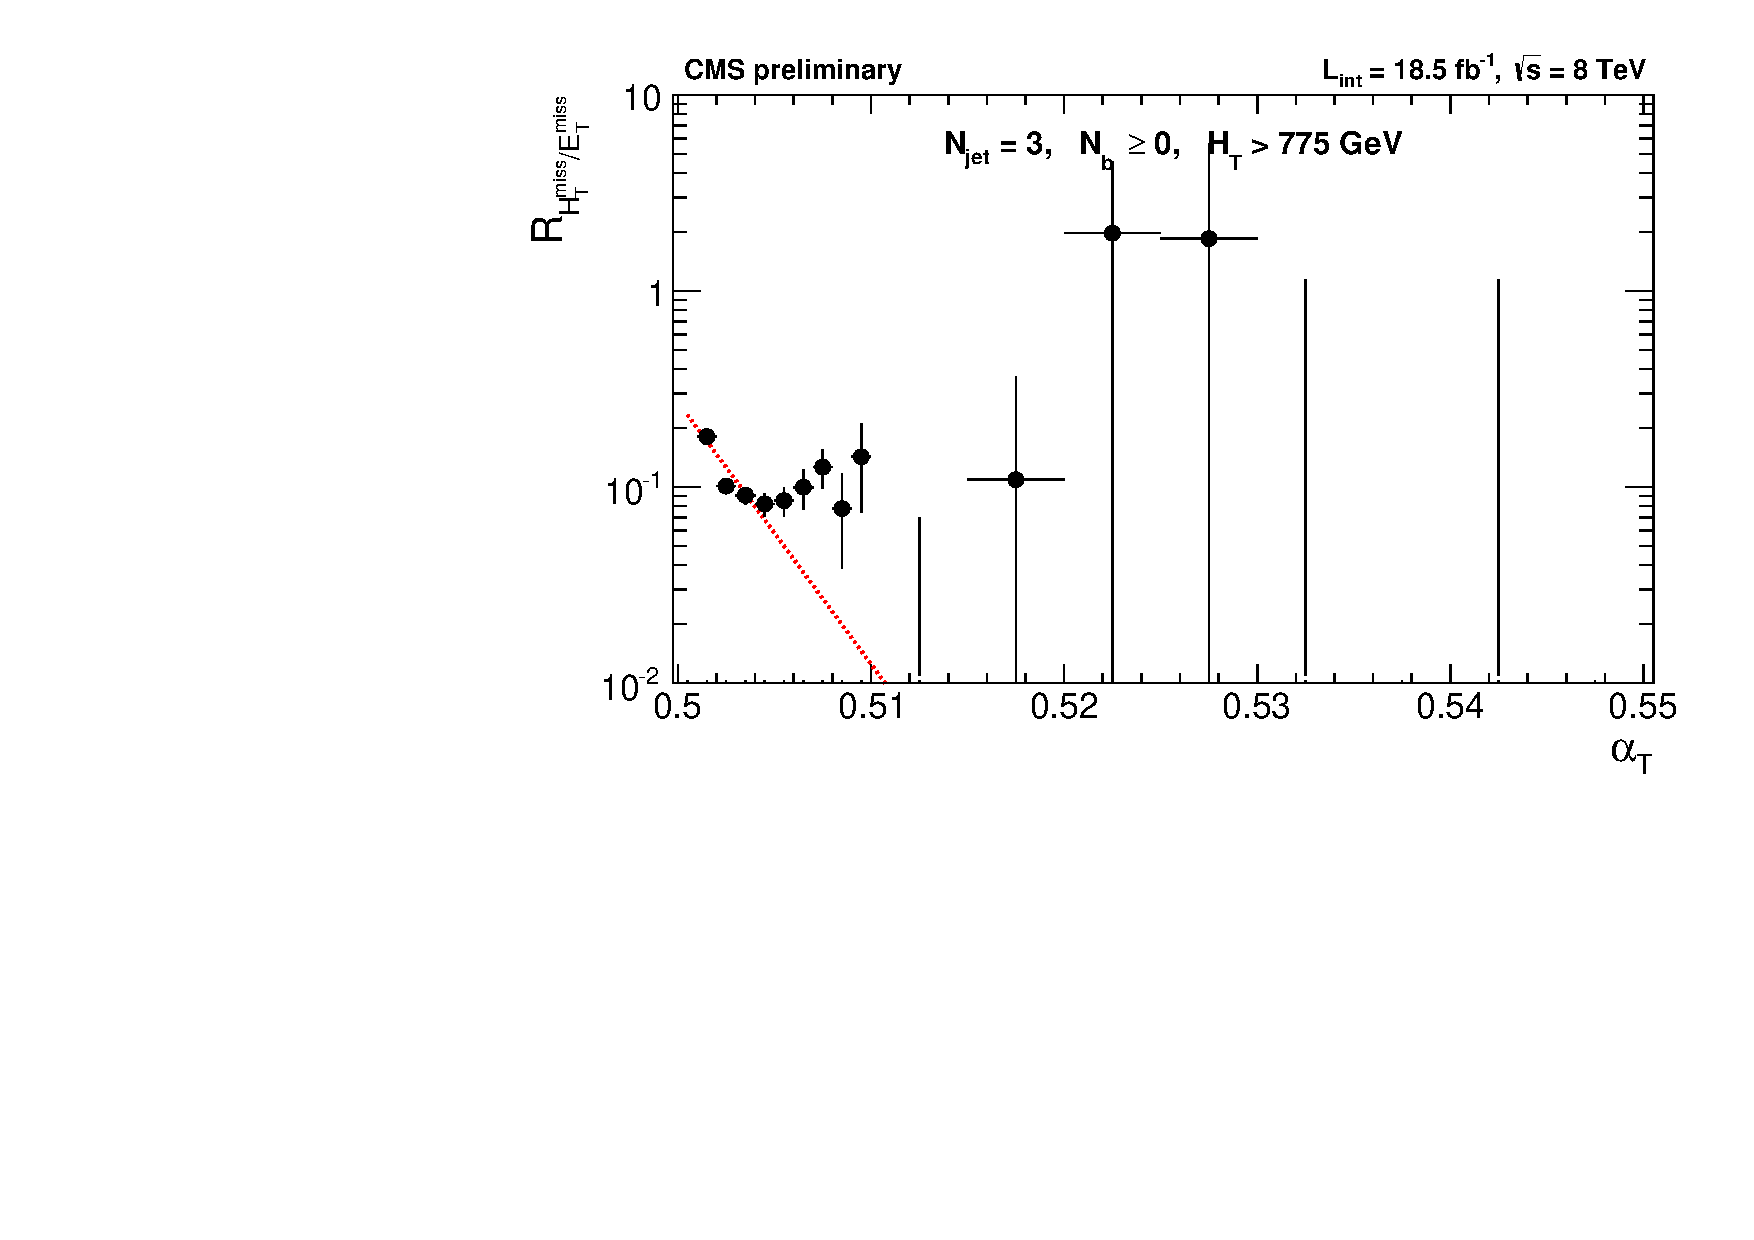
\includegraphics[width=\textwidth]{Figs/dphi/chris2/data/dphi_lt0p3/v2/ratio_eq3j_ge0b_775}
      \caption{Data, $\nj = 3$, \mindphistar < 0.3}
      \label{fig:rdphi_data_j3_lt0p3}
    \end{subfigure} \\

    \begin{subfigure}[b]{0.46\textwidth}
      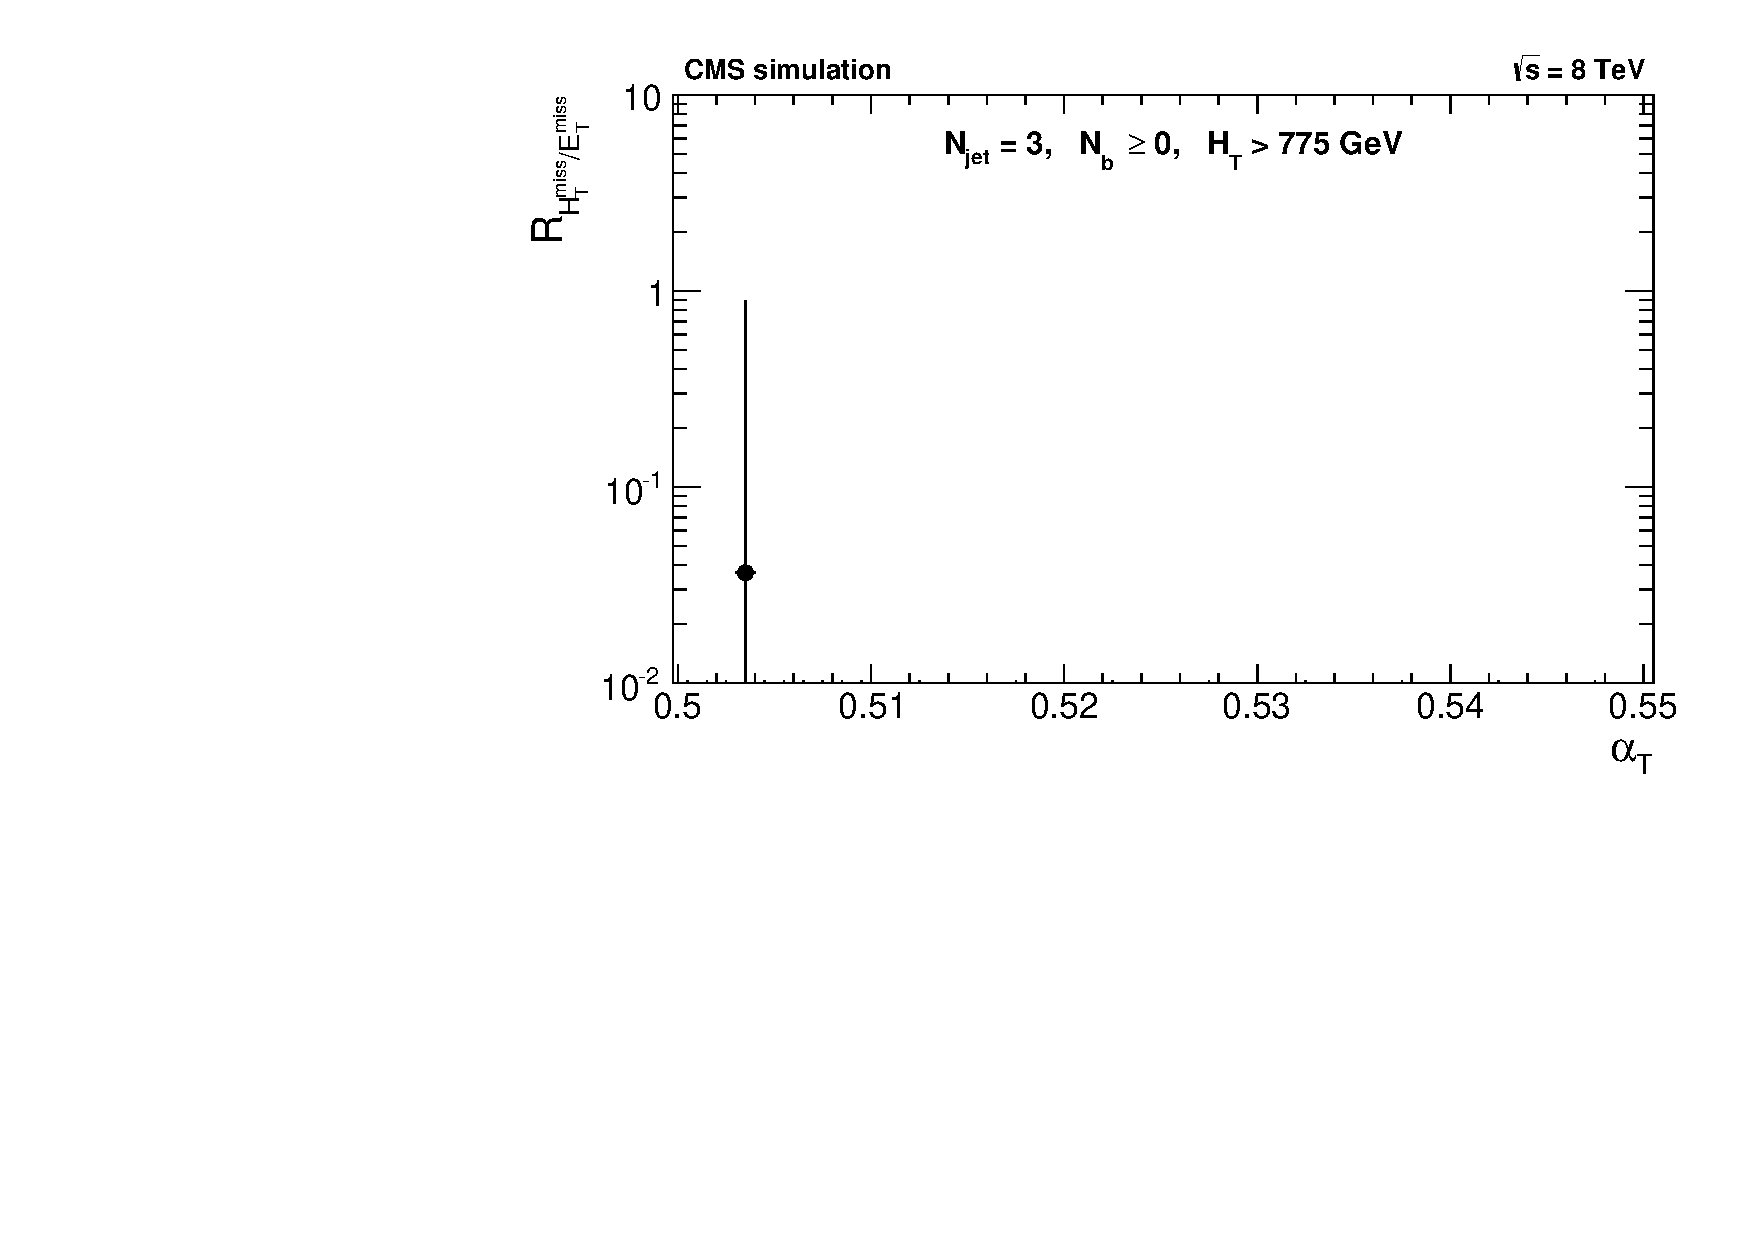
\includegraphics[width=\textwidth]{Figs/dphi/chris2/qcd_mc/dphi_gt0p3/v2/ratio_eq3j_ge0b_775}
      \caption{Simulation, $\nj = 3$, \mindphistar > 0.3}
      \label{fig:rdphi_sim_j3_gt0p3}
    \end{subfigure}
    \begin{subfigure}[b]{0.46\textwidth}
      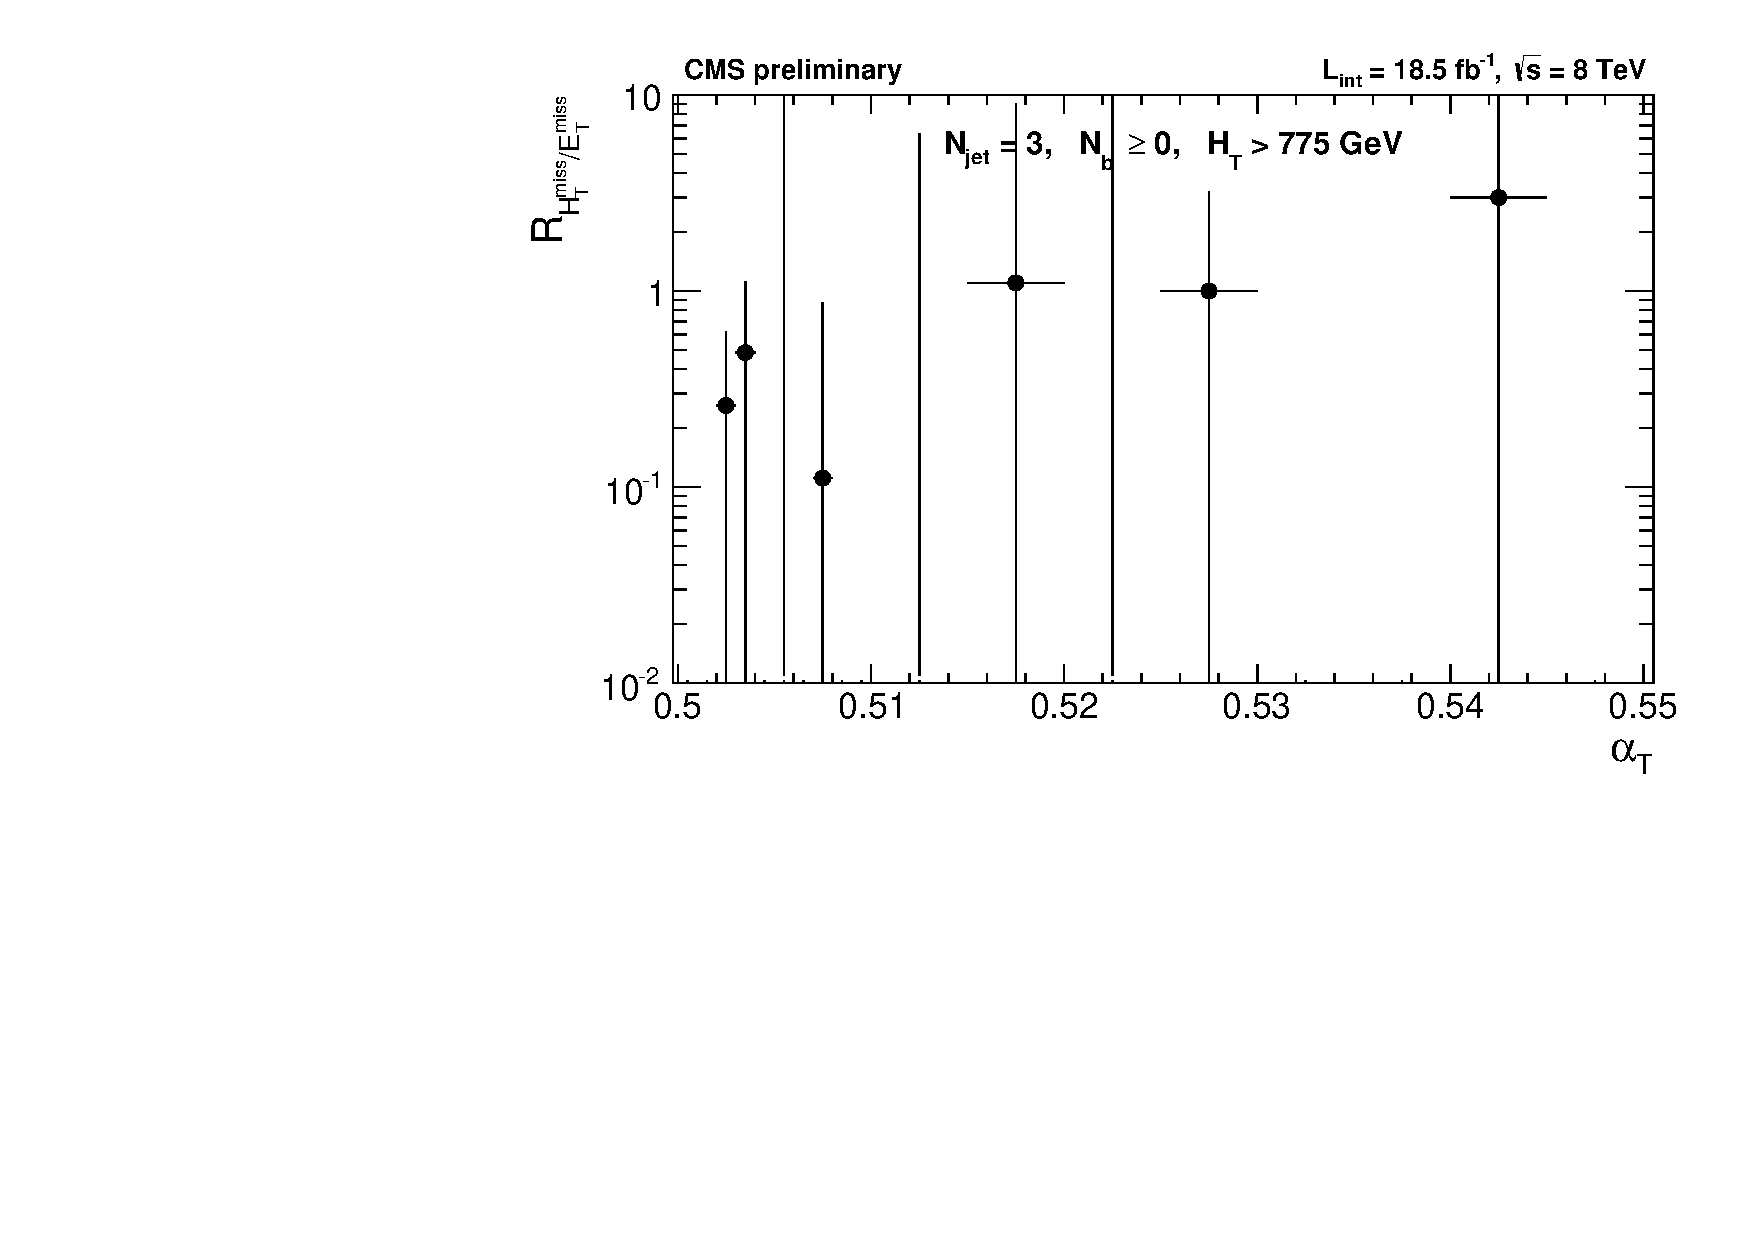
\includegraphics[width=\textwidth]{Figs/dphi/chris2/data/dphi_gt0p3/v2/ratio_eq3j_ge0b_775}
      \caption{Data, $\nj = 3$, \mindphistar > 0.3}
      \label{fig:rdphi_data_j3_gt0p3}
    \end{subfigure} \\

    \begin{subfigure}[b]{0.46\textwidth}
      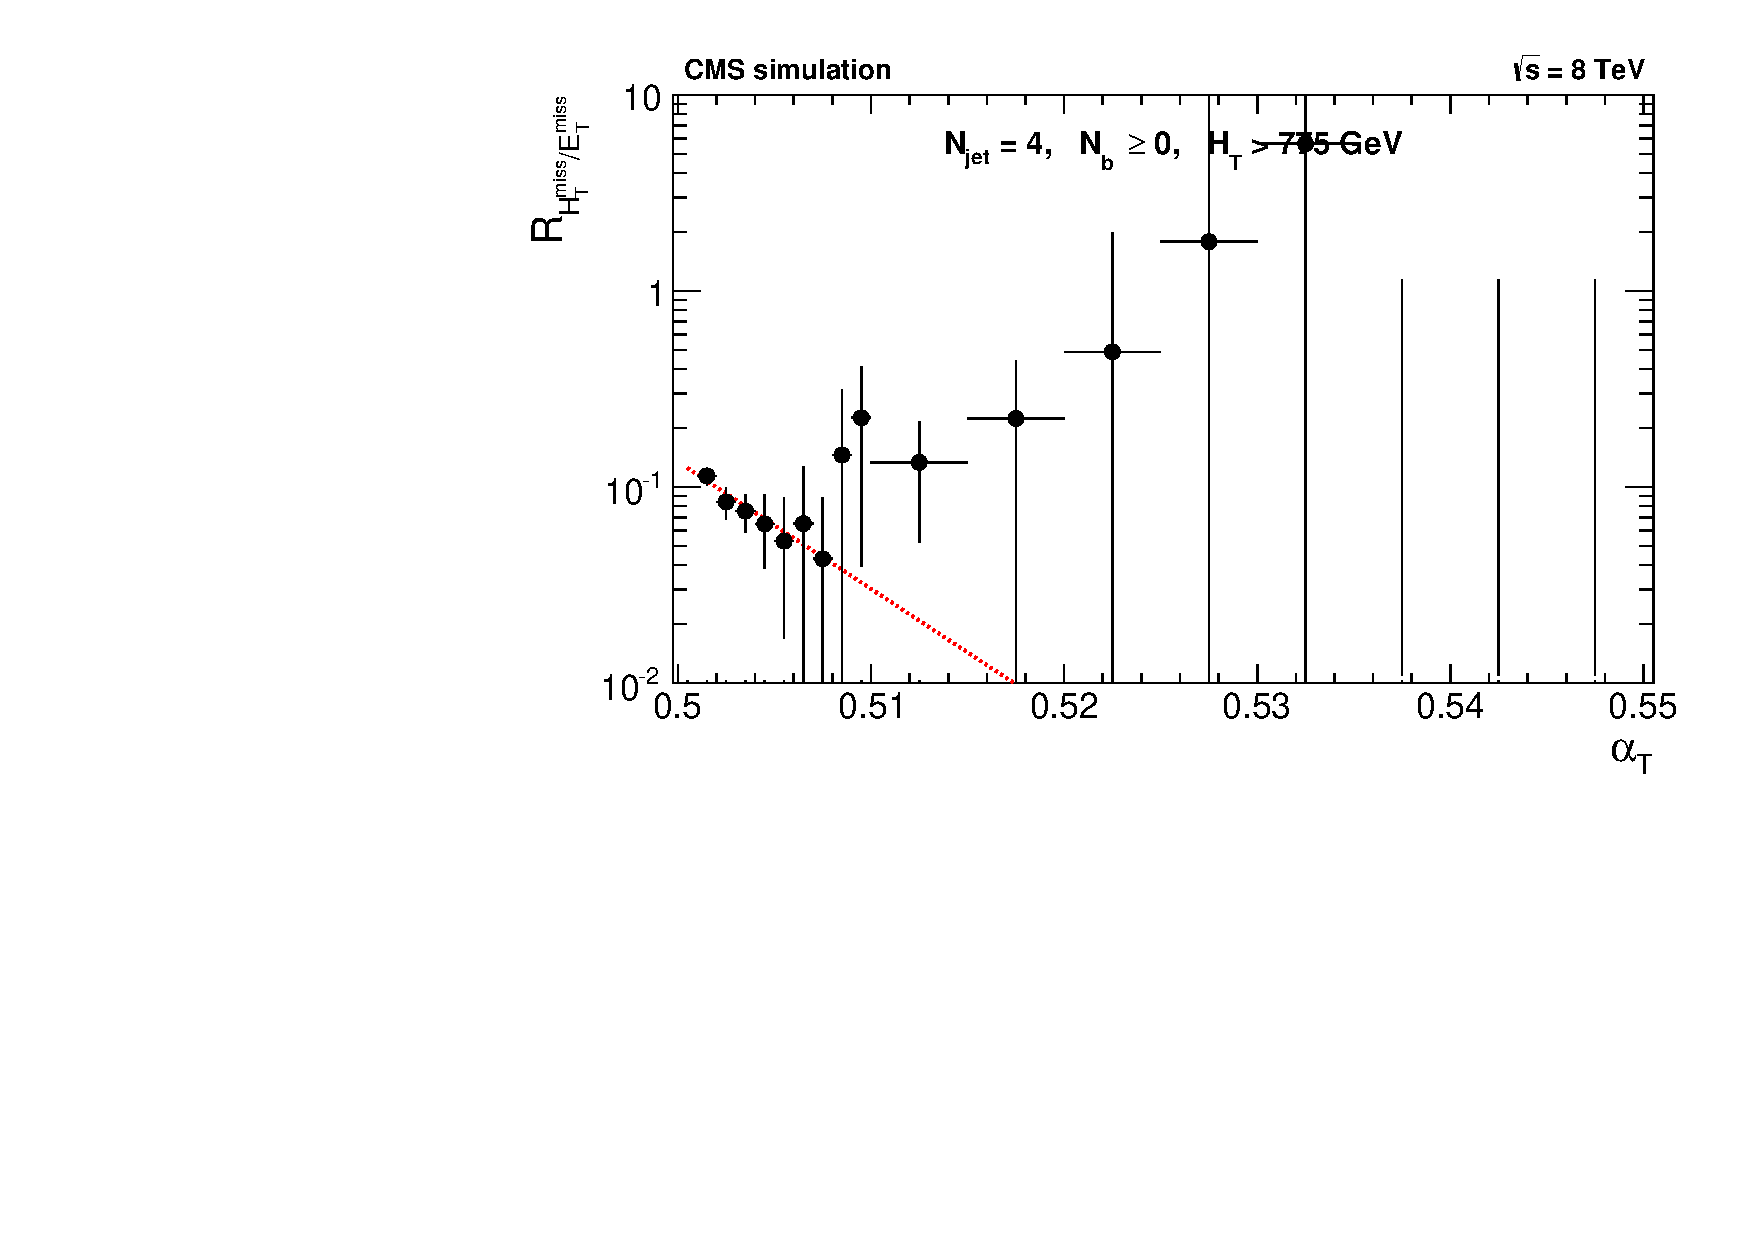
\includegraphics[width=\textwidth]{Figs/dphi/chris2/qcd_mc/dphi_lt0p3/v2/ratio_eq4j_ge0b_775}
      \caption{Simulation, $\nj = 4$, \mindphistar < 0.3}
      \label{fig:rdphi_sim_j4_lt0p3}
    \end{subfigure}
    \begin{subfigure}[b]{0.46\textwidth}
      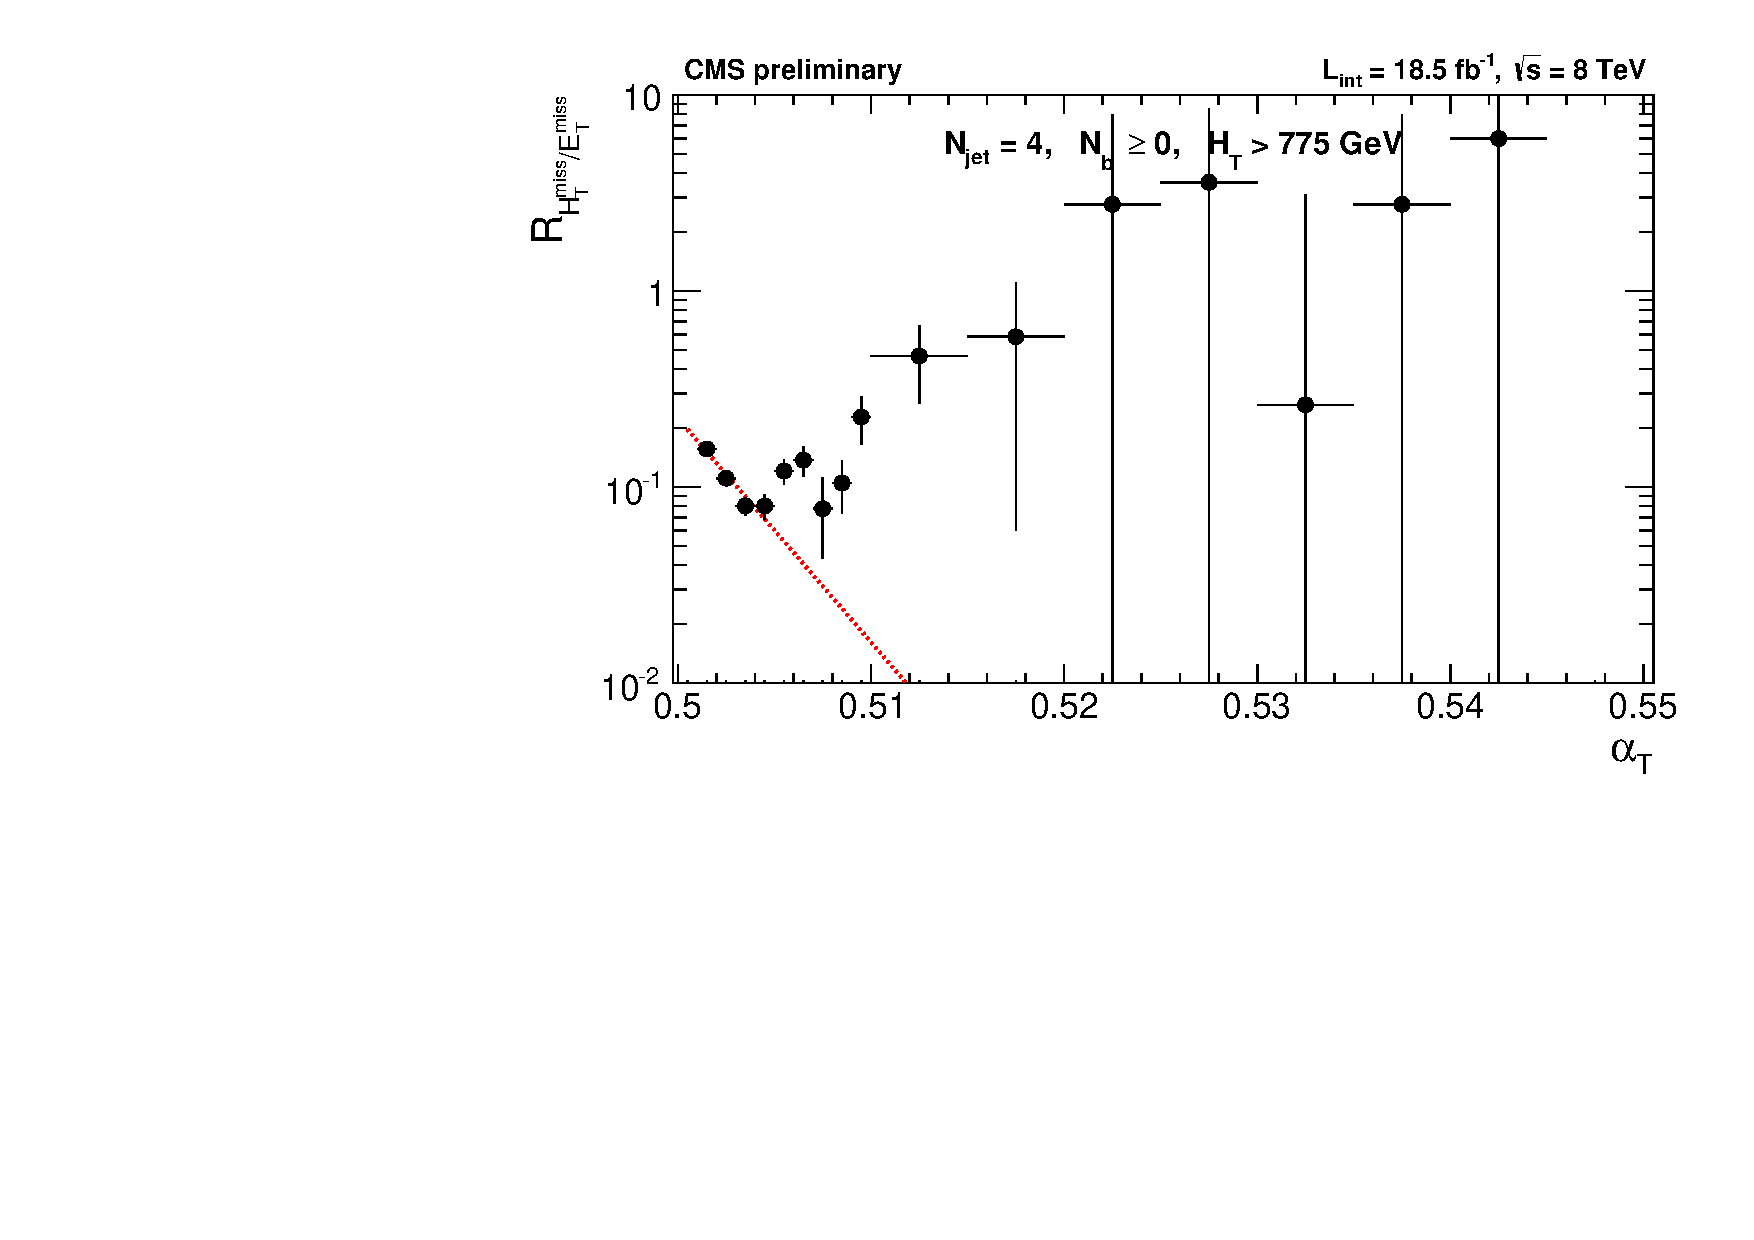
\includegraphics[width=\textwidth]{Figs/dphi/chris2/data/dphi_lt0p3/v2/ratio_eq4j_ge0b_775}
      \caption{Data, $\nj = 4$, \mindphistar < 0.3}
      \label{fig:rdphi_data_j4_lt0p3}
    \end{subfigure} \\

    \begin{subfigure}[b]{0.46\textwidth}
      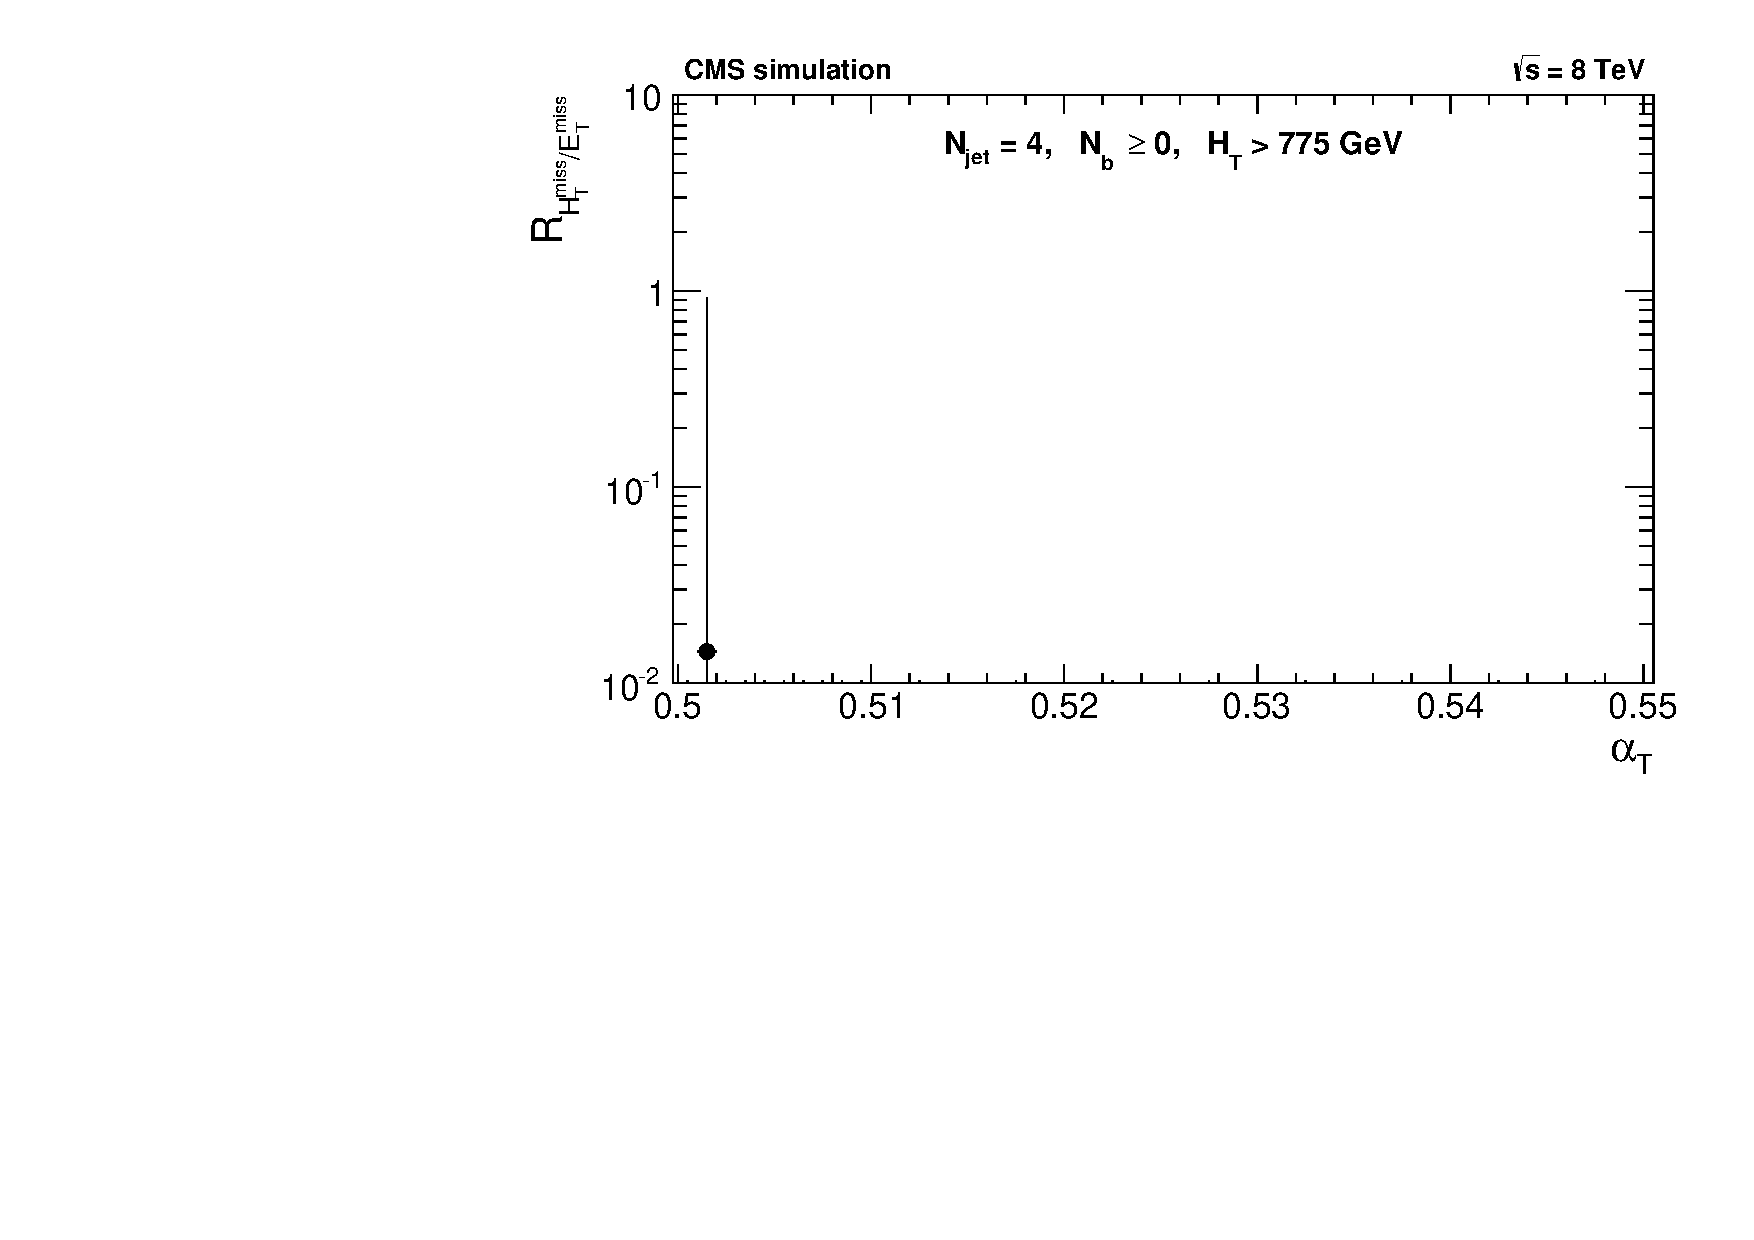
\includegraphics[width=\textwidth]{Figs/dphi/chris2/qcd_mc/dphi_gt0p3/v2/ratio_eq4j_ge0b_775}
      \caption{Simulation, $\nj = 4$, \mindphistar > 0.3}
      \label{fig:rdphi_sim_j4_gt0p3}
    \end{subfigure}
    \begin{subfigure}[b]{0.46\textwidth}
      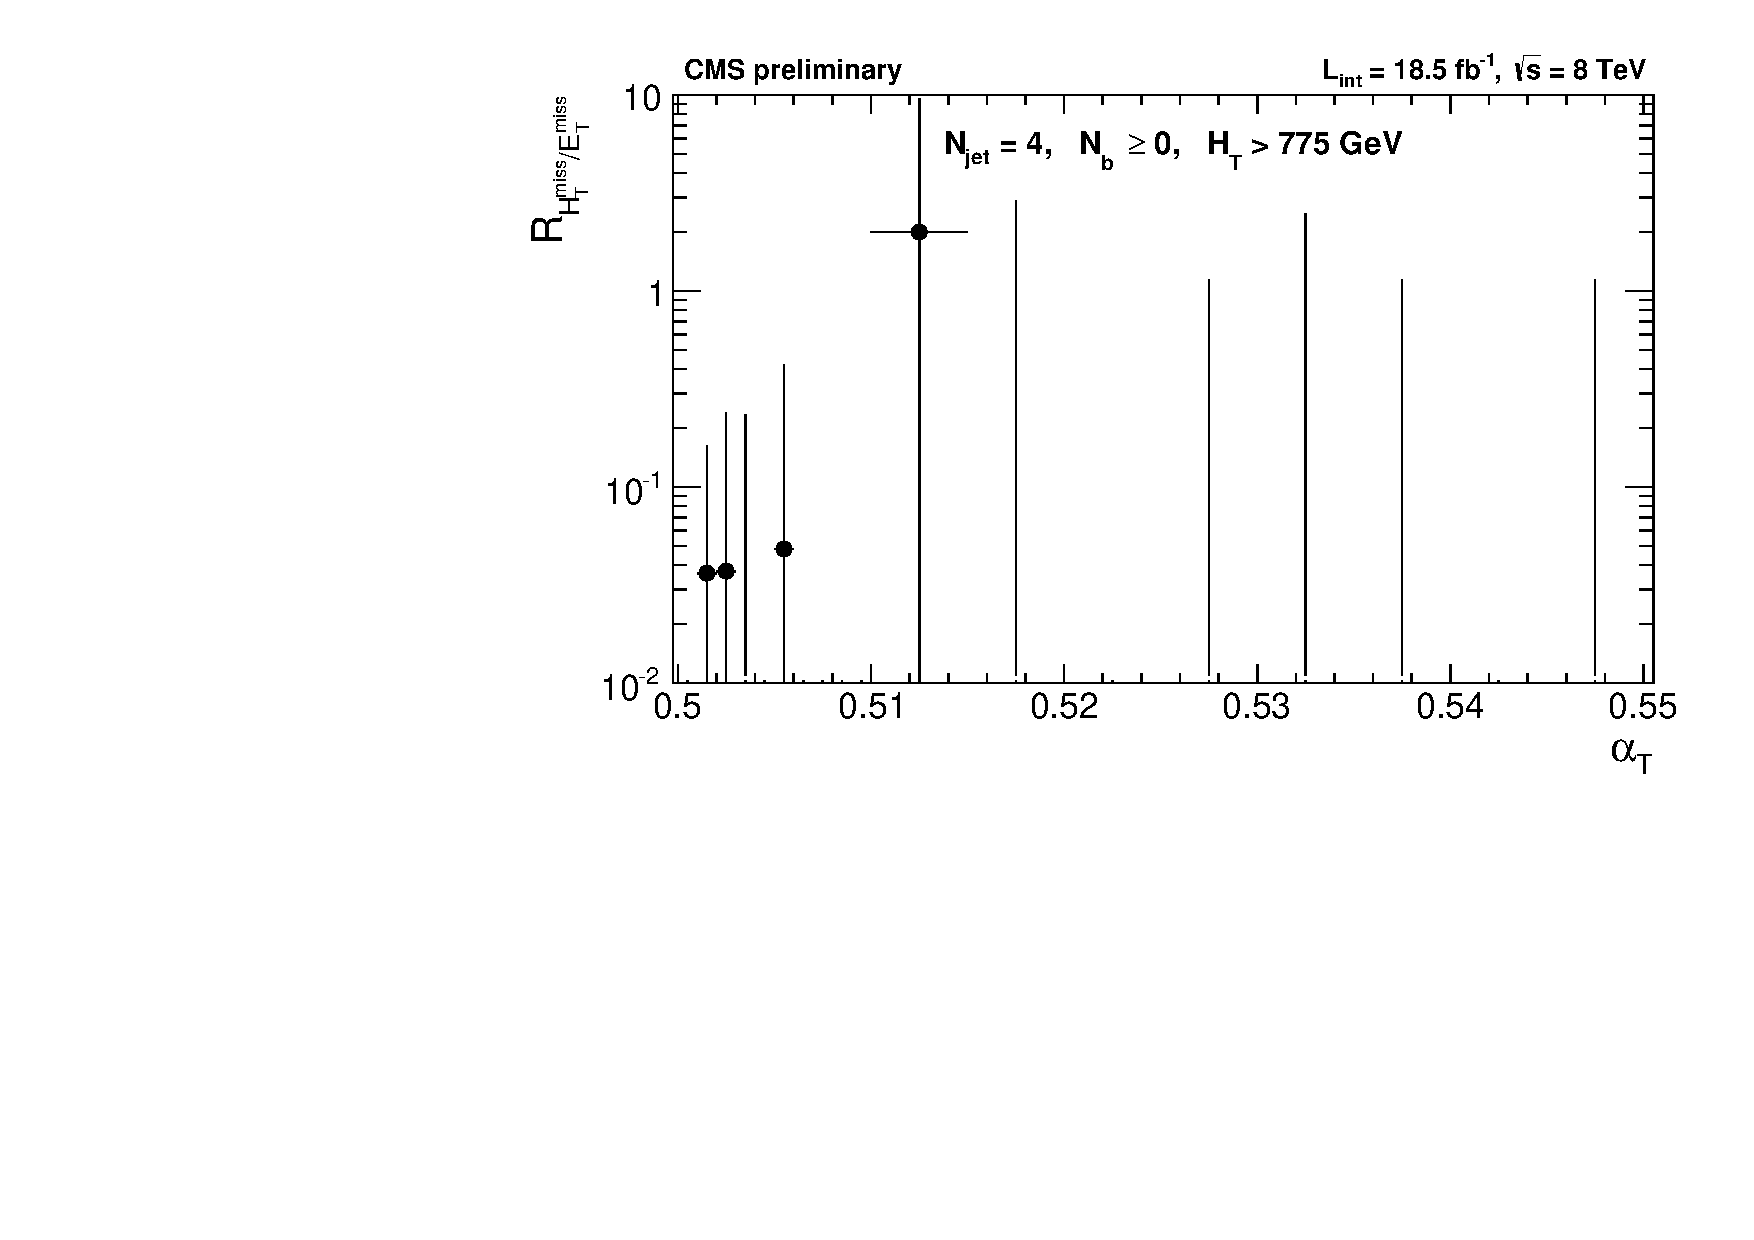
\includegraphics[width=\textwidth]{Figs/dphi/chris2/data/dphi_gt0p3/v2/ratio_eq4j_ge0b_775}
      \caption{Data, $\nj = 4$, \mindphistar > 0.3}
      \label{fig:rdphi_data_j4_gt0p3}
    \end{subfigure}
    \caption{Ratio of events passing and failing the \mhtmet < 1.25
    requirement, both for simulation (left column) and data (right column).
    Individual plots are shown for all combinations of $\nj = 3$ or $\nj = 4$,
    and \mindphistar > 0.3 or \mindphistar < 0.3. Note that data plots
    represent events counts after the EWK background prediction has been
    subtracted.}
    \label{fig:rmhtmet_dphi_data_sim}
  \end{figure}

When the QCD-enriched \mindphistar < 0.3 region is considered, for low \alphat
values the ratio \rmhtmet is seen to fall exponentially. However at
higher \alphat values, where the bulk of QCD events are rejected, the
constant pedestal arises due to heavy-flavour QCD jets. Inverting
the \mindphistar requirement reduces the pedestal to entirely negligible
levels. Similarly to figure~\ref{fig:data_pred_dphistar_eff}, data counts are
corrected to remove the EWK background prediction and so gain a reasonably
large uncertainty, however still agree statistically with zero.

As a consequence of these studies of events with jets containing sources of
genuine \met jet, the analysis
additionally requires that all events have \mindphistar > 0.3 in the signal
region. The effect of this requirement on signal efficiency for the models 
considered in this thesis are discussed in appendix~\ref{ch:app_dphistar}.

% For bins of $\HT>375$~\gev the leading two jets in the event are required to 
% have $\Pt>100$~\gev, with all additional jets having half the requirement of
% $\Pt>50$~\gev. In order to maintain a similar kinematic phase space throughout
% the many \HT bins, these jet \Pt requirements are scaled for the lower \HT bins 
% as shown in Table~\ref{tab:analysis_thresholds}.


\section{Example distributions and cutflow}

Example distributions from MC simulations of \alphat, \HT, \mht and jet \Pt  are
shown in figure~\ref{fig:datamc_had_inc}. Example cutflow yields are shown in
table~\ref{tab:had_data_cutflow} for data in the \HT > 375~\gev region, with an
inclusive selection on \nj and \nb.


\begin{figure}[!ht]
  \centering
    \begin{subfigure}[b]{0.48\textwidth}
      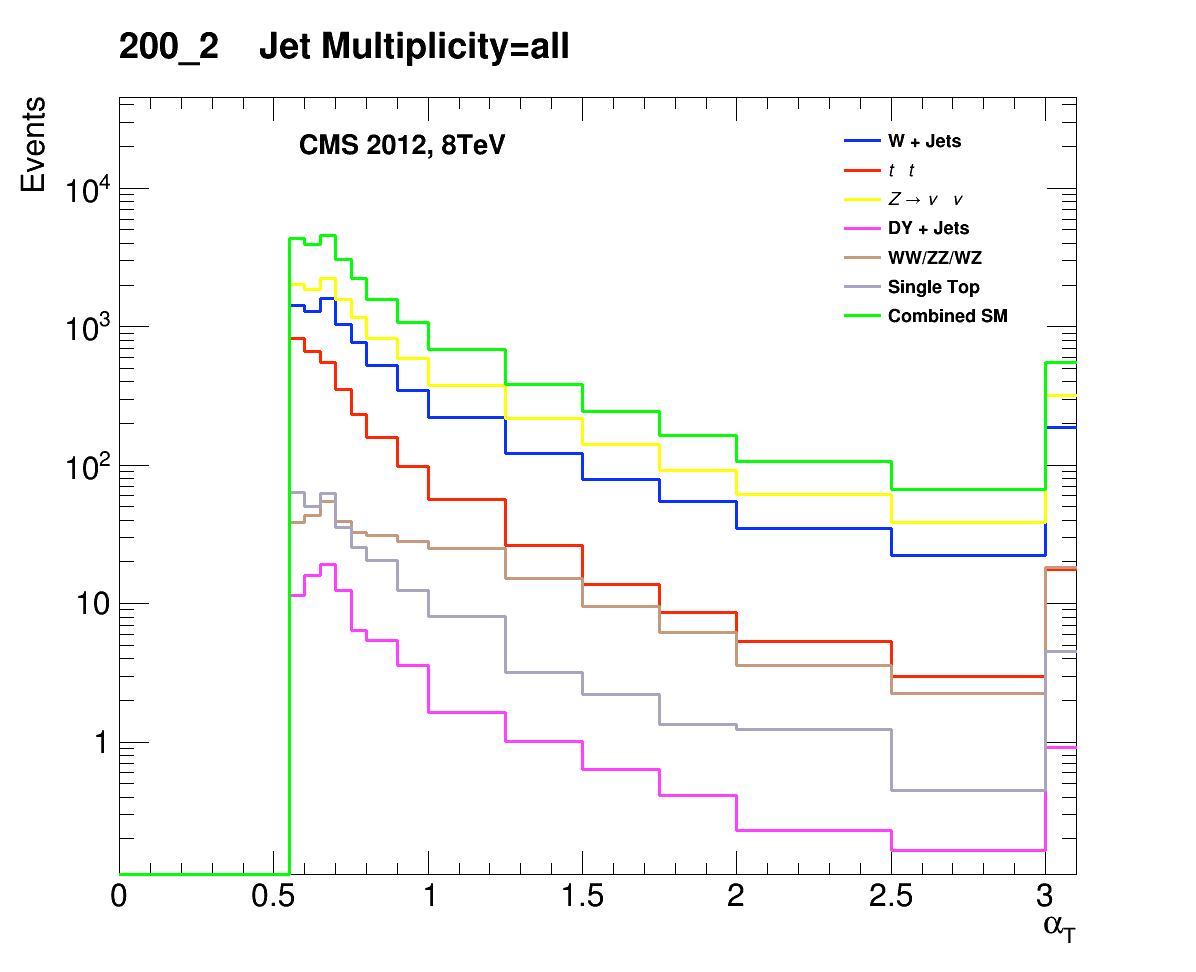
\includegraphics[width=\textwidth]{Figs/datamc/had/v1/AlphaT_all_200_upwards}
      \caption{\alphat}
    \end{subfigure}
    \begin{subfigure}[b]{0.48\textwidth}
      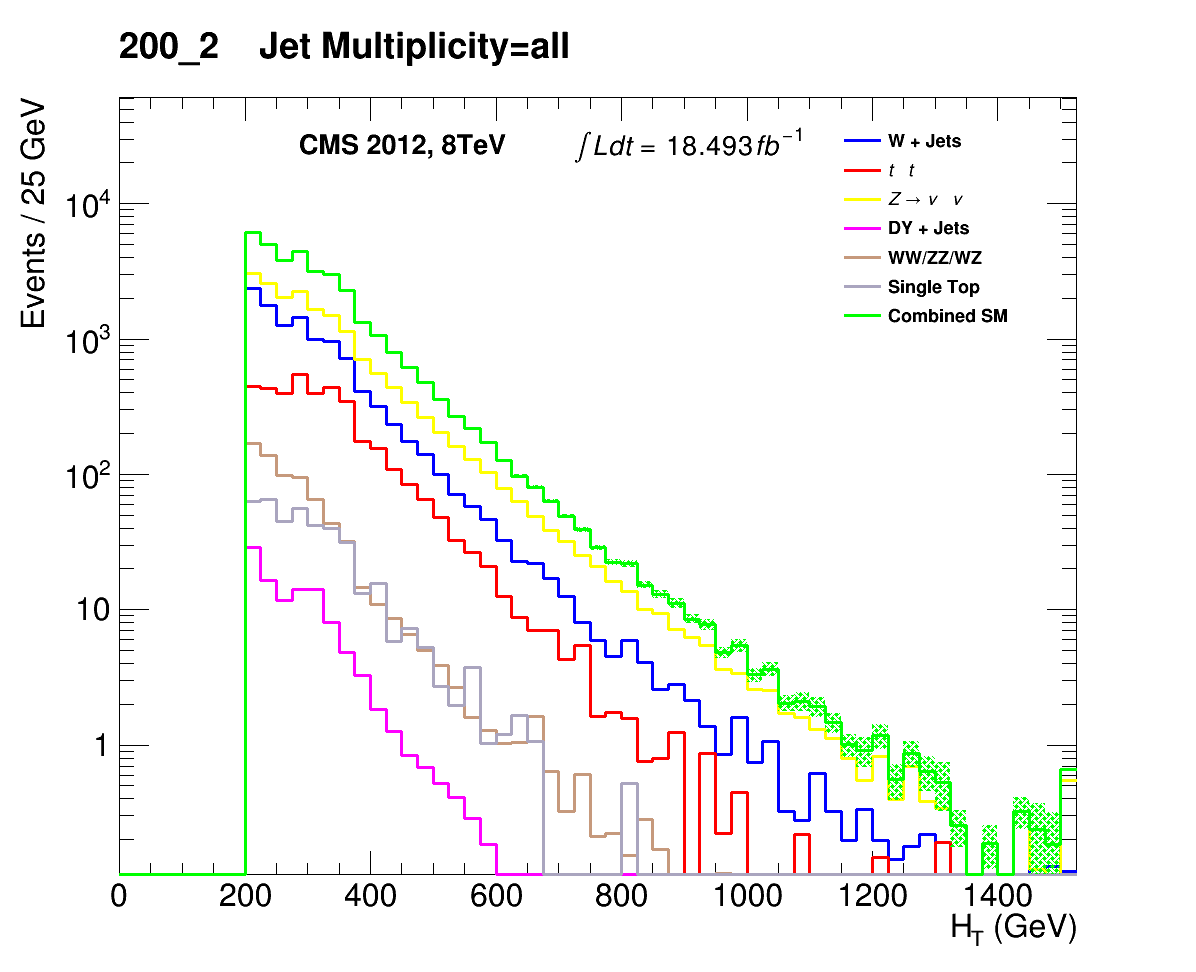
\includegraphics[width=\textwidth]{Figs/datamc/had/v1/HT_all_200_upwards}
      \caption{\HT}
    \end{subfigure} \\
    \begin{subfigure}[b]{0.48\textwidth}
      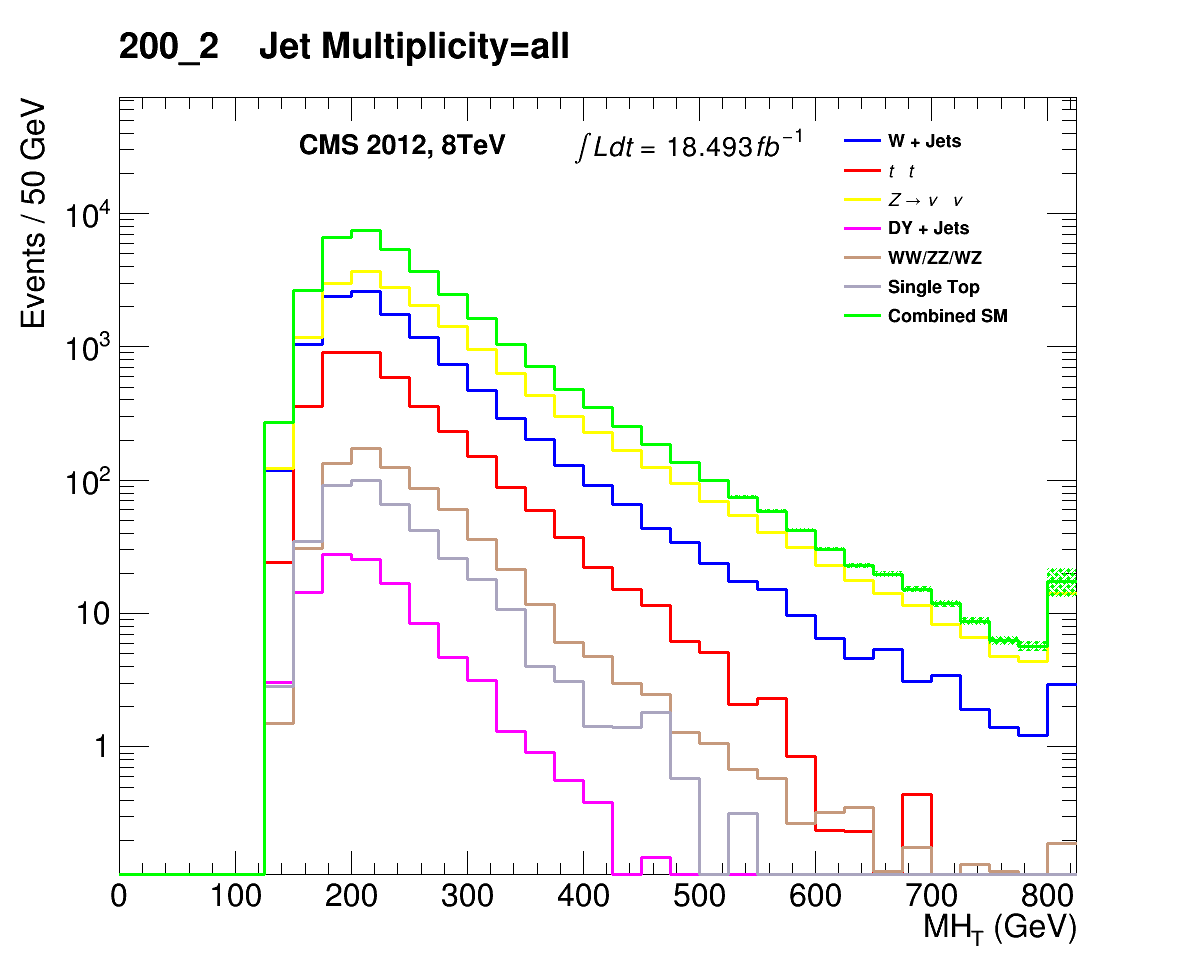
\includegraphics[width=\textwidth]{Figs/datamc/had/v1/MHT_all_200_upwards}
      \caption{\mht}
    \end{subfigure}
    \begin{subfigure}[b]{0.48\textwidth}
      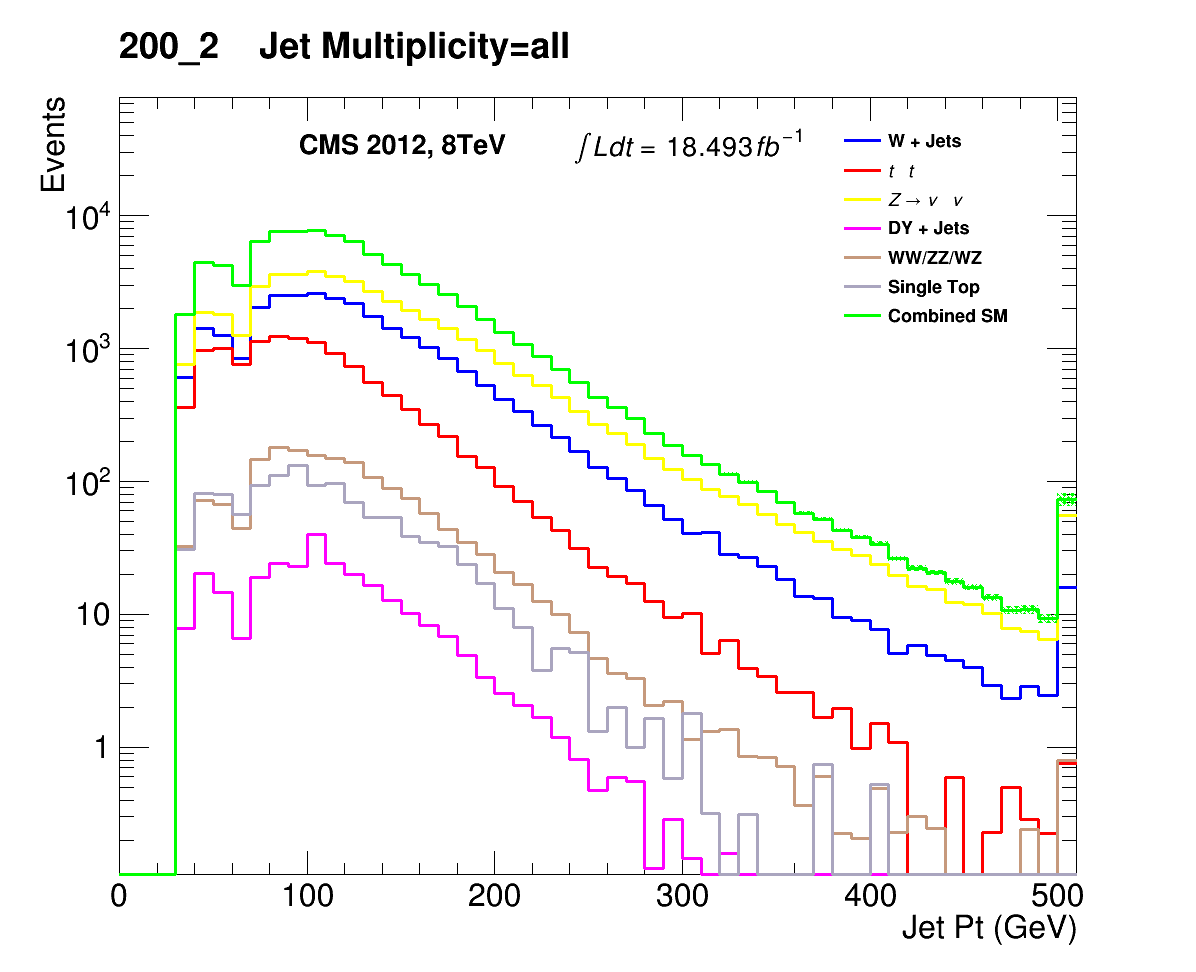
\includegraphics[width=\textwidth]{Figs/datamc/had/v1/CommonJetPt_all_200_upwards}
      \caption{Jet \Pt}
    \end{subfigure} \\
    \caption{\label{fig:datamc_had_inc}
    MC distributions for the full hadronic signal selection. The 
    sum of the individual sample contributions is shown in green. Plots
    are for $\HT>200$~\gev, $\nj\geq2, \nb\geq0$.
    }
\end{figure}

\begin{table}[ht!]
  \caption{The cutflow of the hadronic selection in data. The subscript `fail'
  indicates an object which did not meet all ID requirements, and so is not
  considered as a `common object'. The event selection follows an inclusive
  selection in data of $\HT > 375$~\gev, $\nj \geq 2$ and $\nb \geq 0$. }
  \label{tab:had_data_cutflow}
  \centering
  \footnotesize
  \begin{tabular}{ lcc }
    \hline
    \hline
    Cut    & Eff (\%) & N \\
    \hline
  Event Count  & 100.00  & 161866108 \\
  Good Event JSON Filter  & 94.97  & 153716716 \\
  $\nj \geq 2$  & 98.68  & 151689664 \\
  MET Filters & 98.81  & 149885013 \\
  Vertex Noise Filter & 99.91  & 149746017 \\
  DeadECAL Filter & 35.44  & 53066597 \\
  Select seed Trigger & 3.76  & 1995549 \\
  $n_{e} = 0$ & 98.48  & 1965269 \\
  $n_{\gamma} = 0$  & 97.70  & 1920124 \\
  $n_{\mu} = 0$ & 98.36  & 1888711 \\
  $\text{EMF}_{max}$ for all jets > 0.1 & 99.99  & 1888576 \\
  Leading jet \Pt > 100~\gev  & 97.83  & 1847501 \\
  Leading jet $\eta$ < 2.5  & 97.31  & 1797777 \\
  Sub-Leading jet \Pt > 100~\gev  & 81.75  & 1469654 \\
  $n_{jet, fail} = 0$ & 81.73  & 1201096 \\
  $\Delta R(\mu^i_{fail}, jet^j) < 0.5$ & 98.77  & 1186370 \\
  $(\sum_{}^{n_{vertices}}{\Pt}$) / \HT & 100.00  & 1186368 \\
  recHitCut & 98.44  & 1167861 \\
  $n_{SIT} = 0$ & 85.77  & 1001646 \\
  \mindphistar > 0.3  & 19.50  & 195361 \\
  \HT > 375~\gev  & 73.33  & 143255 \\
  \mhtmet < 1.25  & 9.26  & 13263 \\
  \alphat > 0.55  & 38.25  & 5073 \\
    \hline
    \hline
  \end{tabular}
\end{table}






